\documentclass[draft]{Feb-3-22-latex-templates/agujournal2019}

% --- Journal Provided
\usepackage{url}
\usepackage{lineno}
\usepackage{soul}
\journalname{Journal of Advances in Modeling Earth Systems (JAMES)}
\draftfalse
\linenumbers

% --- Custom additions
\usepackage{amsmath, amssymb}
\usepackage{mathtools} % for \coloneqq
\usepackage{color}
\usepackage{graphicx}
\usepackage{natbib}
\usepackage[capitalise]{cleveref}
\usepackage{bm}

\newcommand{\red}[1]{\textcolor{red}{#1}}
\newcommand{\blue}[1]{\textcolor{blue}{#1}}
\usepackage{oden}

% Removes redundant "appendix"
\crefname{appendix}{}{}

\begin{document}

% --- Header
\title{A Practical Gaussian Covariance Formulation for Applications with
       Anisotropic and Nonstationary Fields}
\authors{Timothy A. Smith\affil{1,2,3}, Patrick Heimbach\affil{3,4,5}}

\affiliation{1}{CIRES}
\affiliation{2}{PSL}
\affiliation{3}{Oden}
\affiliation{4}{UTIG}
\affiliation{5}{JSG}

% --- Key points, abstract, plain language summary
\begin{keypoints}
    \item We derive a generic covariance model appropriate for anisotropic,
        nonstationary fields \red{This is the title...}
    \item The formulation presents a number of computational advantages compared
        to previous work, such as easy application of to both the covariance or
        precision operators (its inverse)
    \item Numerical experiments agree well with theory... \red{more on this...}
\end{keypoints}

\begin{abstract}
\end{abstract}

\section*{Plain Language Summary}
Mat\'ern, Weaver, and Courtier walk into a bar...

\section{Introduction}
\label{sec:intro}
A fundamental requirement for the inverse problem that we address in this work
is the specification of a prior distribution, $\priorDist(\params)$.
Recall from chapter XX that the multivariate control vector
$\params$ consists of the
potential temperature, salinity, and zonal velocity at the western boundary of
the domain:
$\params \coloneqq [\thetaParams^T,\saltParams^T,\uvelParams^T]^T \in\paramSpace$.
As is common in large scale geophysical inverse problems, we specify the prior
distribution for the control vector
to be Gaussian: $\priorDist(\params) \coloneqq \mathcal{N}(\params_0, \priorCovMat)$.

Our first objective in the inverse problem is to specify the prior
covariance $\priorCovMat$.
To do this, we obtain univariate prior covariances for
each individual field: $\thetaPriorCovMat$, $\saltPriorCovMat$,
$\uvelPriorCovMat$, which are then stacked block-diagonally to form
$\priorCovMat$ (see below for details).
Our primary focus in this chapter is to describe the generic formulation for
each of these univariate covariance matrices.
To facilitate the discussion, we refer to a generic univariate control variable
$\uni(\x)$ (or $\unis$ upon discretization), which in our specific case is a
placeholder for temperature, salinity, and zonal velocity, and is similarly
applicable to other inverse problems.
We use the general methodology outlined here to specify a prior covariance in
chapter XX.

In oceanographic inverse problems, covariance models must address at least
these three issues.
\begin{enumerate}
    \item Irregular boundaries imposed by continents
    \item Anisotropy due to the shallow fluid-like nature of the ocean
    \item Multivariate control parameters
\end{enumerate}
It is common to use covariance models based on differential operators in order
to handle irregular boundaries, and the question is then how to address the
other two issues within a differential equation.

A common approach to specifying the prior covariance in oceanographic inverse
problems is based on a generalized
diffusion equation \citep{weaver_correlation_2001}.
In this chapter, we outline an alternative approach that brings some practical
advantages which are discussed in section \ref{sec:matern_discussion}.
%#that has a similar structure to the
%#this model, but employs a version of the differential
%#operator presented in \citet{RSSB:RSSB777}.
%The general methodology is as follows.
We define a differential operator that can be represented by the matrix $C$,
that follows the flexible development from \citet{RSSB:RSSB777}.
We note that the matrix form is used for convenience, but that matrices are
never explicitly formed.
We show that the operator $C$ specifies the covariance matrix $CC^T$, that
is almost identical to a Mat\'ern covariance aside from boundary affects
imposed by $C$.
We then augment this differential operator with a sequence of factors that
are suggested by \citet{weaver_correlation_2001}.
That is, we incorporate the sequence of operations:
$\Sigma X C $, where
\begin{equation*}
    X \coloneqq \text{diag}\left\{ 1/\hat{\sigma}_{i}\right\}_{i=1}^{N}
\end{equation*}
is a
normalization matrix computed from the pointwise marginal variance at grid cell
$i$: $\hat{\sigma}^2_{i}$, and
\begin{equation*}
    \Sigma \coloneqq \text{diag}\left\{\sigma_\uni\right\}_{i=1}^{\nuni}
\end{equation*}
is the specified magnitude of prior uncertainty (standard deviation) for a
generic univariate parameter field $\unis\in\uniSpace$ (e.g.\ initial temperature).
With these definitions, $XCC^TX$ is a correlation matrix, and
\begin{equation}
    \Gamma_\uni \coloneqq \Sigma X C C^T X \Sigma =
    \Gamma_\uni^{1/2}\Gamma_\uni^{T/2}
\end{equation}
defines the covariance for a generic univariate parameter field $\unis$.

The full prior covariance for a general multivariate application is then formed
by specifying individual covariance operators as above, and stacking them
together block diagonally.
To be concrete, the prior covariance for the specific inverse problem in this
work, i.e. for the steady state temperature, salinity,
and velocity fields at the open boundary of the computational domain,
is formulated as
\begin{equation*}
    \priorCovMat \coloneqq
    \begin{pmatrix}
        \thetaPriorCovMat & & \\
        & \saltPriorCovMat & \\
        & & \uvelPriorCovMat \\
    \end{pmatrix} \, .
\end{equation*}
To keep this chapter general, we focus on specifying the covariance for a generic
univariate control parameter, $\uni(\x)$ which can be considered a placeholder
for each variable temperature, salinity, and velocity separately.
We wait until
chapter xx to discuss the specification of the prior
for each parameter, as this is becomes specific to our application.
Finally, we note that nonzero off diagonal terms in $\priorCovMat$ above (or an
additional operator) could be used to specify cross covariance between each
variable.
We consider this future work, and discuss potential options in
section XX.

In the following sections we review the general Mat\'ern type covariance
form that is suggested by \citet{RSSB:RSSB777}.
We then develop the differential operator, $C$, that
forms the backbone of our covariance model.
We show that our numerical implementation of the covariance model produces correlation
length scales that are expected from the analysis in section
\ref{sec:matern_operator}.
We conclude by discussing some advantages that this approach offers.


\section{Mathematical Context and Background}
\label{sec:review}

In order to provide some mathematical context for our correlation model
developments, we first outline the generic inverse problem that is central to
a variety of applications such as numerical weather prediction and state
estimation.
Our notation closely follows \citet{ide_unified_1997}, and we note that matrix
notation is used to describe the problem, but these matrices are never formed
explicitly.
Rather, all matrices presented are described by operators that can be applied
scalably in high dimensional inverse problems.
We then review correlation models that are based on the application of a
diffusion operator \citep{weaver_correlation_2001,mirouze_representation_2010},
which are commonly used for large scale geophysical inverse problems
\citep[e.g.][]{forgetECCOv4,moore_regional_2011-1}.
We then discuss the developments from \citet{RSSB:RSSB777}, outlining the
connection between the solution to a Stochastic PDE (SPDE) and a Gaussian random
field with Mat\'ern type covariance.
We finish by showing a comparison of auto-regressive and the more general
Mat\'ern type correlation functions with a classical Gaussian.
These comparisons motivate our development of an anistropic, nonstationary correlation
model, which is presented in \cref{sec:matern_operator}.


\subsection{Inverse Problem Formulation}
\label{ssec:da_formulation}

We consider the general problem of finding the optimal control vector,
$\params$, which minimizes the regularized model-data misfit cost function
\begin{linenomath*}\begin{equation*}
    \cf(\params) =
        \dfrac{1}{2}||\pto(\params) - \data||_{\obsCovMat^{-1}}^2
        +
        \dfrac{1}{2}||\params - \priorParams||_{\priorCovMat^{-1}}^2 \, .
\end{equation*}\end{linenomath*}
Here $\norm{\mathbf{v}}_A = \sqrt{\mathbf{v}^T A \mathbf{v}}$ is a weighted
Euclidean norm.
The solution to this inverse problem, $\paramsMAP$, arises from a tradeoff between fitting the
observational data, $\data$, via the observation operator, $\pto(\cdot)$,
and minimizing deviations from the background-state $\priorParams$.
This tradeoff is governed by the two error covariances, $\obsCovMat$ and
$\priorCovMat$, which dictate how much deviation is acceptable in either term.
On the one hand, the observational error covariance matrix
$\obsCovMat$ represents our uncertainty
in the observational data, together with our confidence in the model's ability
to represent the observed values.
On the other hand, the background-state covariance matrix $\priorCovMat$
represents our uncertainty in the prior estimate or background state,
$\priorParams$.

To be explicit, we focus on how our correlation model fits into the
background-state error covariance, $\priorCovMat$.
However, we note that the formulation could be used for specifying correlations
between observations in a similar fashion to \citet{guillet_modelling_2019}, but
we leave this for future investigation.
In the general case, the control vector $\params$ could be multivariate,
including initial conditions of the system state, uncertain boundary
conditions, or uncertain parameter fields.
Here we employ the decomposition proposed by
\citet{derber_reformulation_1999}
in order to separate the multivariate (i.e.\ cross-variable)
covariance relationships from the univariate (i.e.\ assumed
independent) covariance relationships.
Specifically, the background-state covariance is decomposed as follows
\begin{linenomath*}\begin{equation*}
    \priorCovMat \coloneqq \balanceOperator\unbalancedPriorCovMat\balanceOperator^T \,
    ,
\end{equation*}\end{linenomath*}
where $\balanceOperator$ is a balance operator that deals with the
cross-variable correlations.
The matrix $\unbalancedPriorCovMat$ describes the covariance for the unbalanced
variables and has a block-diagonal structure, such that each
covariance is described independently.
The unbalanced covariance is further factored as
\begin{linenomath*}\begin{equation*}
    \unbalancedPriorCovMat \coloneqq \Sigma \mathcal{C} \Sigma
\end{equation*}\end{linenomath*}
where $\Sigma$ is a diagonal scaling matrix, containing the desired pointwise
standard deviation values and $\mathcal{C}$ is a block diagonal correlation matrix,
describing each variable's independent correlation structure.
To be concrete, this can be viewed as
\begin{linenomath*}\begin{equation*}
    \unbalancedPriorCovMat =
    \begin{pmatrix}
        \Sigma_\alpha\corrMat_\alpha\Sigma_\alpha & 0 & \cdots & 0 \\
        0 & \Sigma_\beta\corrMat_\beta\Sigma_\beta & \cdots & 0 \\
        0 & 0 & \ddots & 0  \\
        0 & 0 & \cdots & \Sigma_\gamma\corrMat_\gamma\Sigma_\gamma \\
    \end{pmatrix}
\end{equation*}\end{linenomath*}
where $\alpha, \beta, \gamma$ are placeholders for unique variables,
and each $\Sigma_\alpha, \corrMat_\alpha$ pair describes the covariance for its
particular variable ($\alpha$, in this case).
In this formulation, $\corrMat_\alpha$ describes the spatial correlation
structure for the variable $\alpha$, and is scaled to a proper covariance given the
diagonal matrix $\Sigma_\alpha$.

The goal of this paper is to formulate a generic operator for $\corrMat$
that could be
used in a variational data assimilation system to specify
correlations for any variable, e.g.\ $\corrMat_\alpha$, $\corrMat_\beta$, etc.
More specifically, we specify the square root $\corrMat^{1/2}$, such that
$\corrMat = \corrMat^{1/2}\corrMat^{T/2}$.
To provide some additional context for this development,
we first review past work that has achieved this with a generalized
diffusion-based operator.


\subsection{Diffusion Based Correlation Models}
\label{ssec:wc01_review}

A common method for specifying the correlation structure,
$\corrMat$, in variational data assimilation systems, especially in
oceanographic applications, is through the solution of a generalized diffusion
equation,
\begin{linenomath*}\begin{equation}
    \dfrac{\partial \uni}{\partial t} = \nabla \cdot \kappa \nabla\uni \, .
    \label{eq:diffusion}
\end{equation}\end{linenomath*}
Here $\kappa$ is a diffusion tensor that controls anisotropy and
nonstationarity, $t$ is a ``pseudo-time'' coordinate, and the solution to this
equation has a Gaussian, or ``Gaussian-like'', covariance.

Building on work from \citet{derber_global_1989, egbert_topexposeidon_1994,
bennett_generalized_1996},
\citet{weaver_correlation_2001} showed that an explicit, forward Euler solution to
\cref{eq:diffusion} provides a scalable approach to defining correlations in
complex domains.
That is, the solution $\uni(T)$ is given by forward pseudo-time stepping
\begin{linenomath*}\begin{equation}
    \uni(T) = \left( I + \nabla\cdot\kappa\nabla\right)^p \uni(t_0) \, ,
    \label{eq:wc01_diffusion}
\end{equation}\end{linenomath*}
which requires $p$ applications of the operator
\begin{linenomath*}\begin{equation*}
    \edop \coloneqq \left(I+\nabla\cdot\kappa\nabla\right) \, ,
\end{equation*}\end{linenomath*}
where $p$ is chosen in
order to achieve numerical stability \citep[see][for details regarding the
discretized form of this operator, and extensions of the model briefly shown
here]{weaver_correlation_2001}.
The solution $\uni(T)$ is shown to have an approximately Gaussian covariance
structure.
A correlation model is thus defined by estimating the pointwise
variance of $\edop^{p}$, $\hat{\sigma}^2(\x)$, in order to define the normalization
matrix
\begin{linenomath*}\begin{equation*}
    \normalizer \coloneqq \text{diag}\{1/\hat{\sigma}_n\}_{n=1}^{\nuni} \, ,
\end{equation*}\end{linenomath*}
where we use $n$ to refer to each grid cell, such that the correlation matrix is
defined through its square root as
\begin{linenomath*}\begin{equation}
    \corrMat^{1/2}_\text{ED} \coloneqq \normalizer \edop^{p} \, .
\end{equation}\end{linenomath*}

The explicit diffusion-based correlation model as briefly summarized here
directly approximates a Gaussian structure.
However, a limitation of this approach is that in some cases, many
iterations are required to keep the scheme stable (i.e.\ a large value of $p$ is
required in \cref{eq:wc01_diffusion}).
As such, \citet{mirouze_representation_2010} and
\citet{carrier_background-error_2010} developed correlation models based on the
\textit{implicit} solution of \cref{eq:diffusion}:
\begin{linenomath*}\begin{equation}
    \left( I - \nabla\cdot\kappa\nabla\right)^M\uni(T) = \uni(t_0) \, ,
    \label{eq:implicit_diffusion}
\end{equation}\end{linenomath*}
which is unconditionally stable.
In this case, a square-root correlation operator is defined through the
``implicit diffusion operator''
\begin{linenomath*}\begin{equation}
    \idop \coloneqq \left(I - \nabla \cdot \kappa\nabla\right)
\end{equation}\end{linenomath*}
as
\begin{linenomath*}\begin{equation}
    \corrMat^{1/2}_\text{ID} \coloneqq \normalizer \idop^{-M} \, ,
\end{equation}\end{linenomath*}
with $\normalizer$ defined based on the operations that precede it.

\citet{mirouze_representation_2010} provide the theoretical underpinnings for
the implicit diffusion approach, and show details regarding its implementation
in general curvilinear coordinates.
Additionally, the authors show that this correlation model corresponds
with an $M$th order auto-regressive (AR) function,
which is a subclass of
Mat\'ern type correlation models \citep[see][for more description of the
parameters controlling this model]{weaver_diffusion_2013}.
Thus, the correlation model has a more general shape, which in the limit of
$M\rightarrow\infty$, approaches a classical Gaussian structure (see
\cref{ssec:correlation_comparison}).

In this work, we formulate a correlation operator in a similar fashion by
directly parameterizing the
elliptic partial differential equation that corresponds to the more generic
Mat\'ern type correlation (or covariance) structure.
In the following subsections, we provide some background on this general correlation
structure to give our developments some context and motivation.

%is a normlization matrix filled with the pointwise inverse standard deviation of the
%operation $\left(I+\nabla\cdot\kappa\nabla \right)^p W^{-1/2}$.
%This definition ensures that the filter defined by $\corrMat^{1/2}_\text{WC01}$
%preserves variance.
%The tensor, $\kappa$, controls the correlation length scales imposed on the
%random field in question.
%Correlation length scales are isotropic (i.e.\ the same in all directions) and
%stationary (i.e.\ they do not change with spatial location) when $\kappa$ is
%constant such that
%\begin{linenomath*}\begin{equation*}
%    L^2 = 2\kappa T \, ,
%\end{equation*}\end{linenomath*}
%where $T\coloneqq p \Delta t$ is the total ``diffusion'' time and $L$ is the
%desired length scale.
%In general, the diffusion tensor can be formulated to produce anisotropic and
%nonstationary length scales, and applied to spherical domains.
%However, a few subtle issues arise in the numerical its implementation.
%First, the number of timesteps, $p$, required to integrate the diffusion
%equation for numerical stability is somewhat unclear.
%In WC01, a necessary but insufficient stability requirement
%$p > 2 (L/\Delta x)^2$ is given.
%However, in practice uncovering the true required value of $p$ requires some
%guess work, and in our experience is multiplicative factor of this lower bound
%(typically $\sim 3$ for our application).
%Additionally, adjoint-based data assimilation systems based on algorithmic
%differentiation may require additional storage, random access memory, or recomputations in order
%to keep track of intermediate results during the adjoint (i.e.\ reverse) timestepping
%in the diffusion model.
%
%In this work we formulate an operator for $\corrMat_\alpha$ which bypasses these
%issues entirely.
%First, we avoid the issue of having to guess the required time steps for numerical
%stability because the application of our correlation operator amounts to solving an
%elliptic PDE, for which a tolerance can be prescribed more readily.
%Moreover, we show that for practical applications this tolerance can be reliably
%prescribed to be quite high $\bigo(10^{-2})$, such that solving the required
%elliptic PDE is computationally efficient.
%Finally, the operator is self-adjoint and so implementing the covariance model
%within any adjoint based solver is a nonissue.
%To provide some details, we next outline the basis for this Mat\'ern covariance
%model from \citet{RSSB:RSSB777}.


\subsection{Review of the Mat\'ern Correlation Structure}
\label{ssec:matern_review}

%In this section we review the link between an elliptic stochastic partial
%differential equation (SPDE) and Gaussian random fields.
The Mat\'ern covariance function between two points, $\xh_1,\xh_2\in\defdomain =
\ndspace$ can be expressed as:
\begin{linenomath*}\begin{equation}
    c(\xh_1,\xh_2) = \dfrac{\hat{\sigma}^2}{2^{\meandiff-1}
    \mathcal{G}(\meandiff)}
    \Big(\sqrt{\deltah} ||\xh_2-\xh_1||\Big)^\meandiff
    \mathcal{B}_\meandiff
    \Big(\sqrt{\deltah} ||\xh_2-\xh_1||\Big) \, .
    \label{eq:matern_covariance_iso}
\end{equation}\end{linenomath*}
Here
$\mathcal{G}$ is the Gamma function,
$\mathcal{B}_\meandiff$ is the modified
Bessel function of the second kind and order $\meandiff$,
$\deltah>0$ is a scaling parameter, and $\meandiff>0$
controls the mean-square differentiability of the underlying statistical process
described by the Mat\'ern covariance.
We note that in the limit of $\meandiff\rightarrow\infty$, the Mat\'ern-type
covariance becomes a classical Gaussian.
Throughout, we refer to a ``Mat\'ern field'' as any normally distributed field that has
covariance described by the Mat\'ern covariance function,
\cref{eq:matern_covariance_iso}.
Additionally, we note that this analytical function only pertains to fields where the
assumptions of stationarity (i.e.\ no spatial dependence) and isotropy (i.e.\ no
directional dependence) hold, and we use notation with ``hats'' $(\hat{\cdot})$
when this is the case.
The marginal variance of such a Mat\'ern field has the analytical form
\begin{linenomath*}\begin{equation}
    \hat{\sigma} = \dfrac{\mathcal{G}(\meandiff)}{
        \mathcal{G}(\meandiff + \ndims/2)
        \deltah^{\meandiff}
        (4\pi)^{\materndim/2}
    } \, ,
    \label{eq:matern_variance}
\end{equation}\end{linenomath*}
where $\ndims$ is the dimensionality of the field being described.
and thus the Mat\'ern covariance can be described via a correlation
function, $r(\xh_1, \xh_2)$, that is scaled by the marginal variance:
\begin{linenomath*}\begin{equation*}
    c(\xh_1, \xh_2) = \hat{\sigma}\,r(\xh_1, \xh_2) \, .
\end{equation*}\end{linenomath*}
%where, to be explicit,


The key relationship discussed in \citet{RSSB:RSSB777} is that any discrete solution to
the elliptic SPDE,
\begin{linenomath*}\begin{equation}
    \Big(\deltah - \nablah\cdot\nablah\Big)^{M}\hat{\uni}(\xh) =
    \Wh(\xh) \, ,
    \label{eq:spde_iso}
\end{equation}\end{linenomath*}
is a Mat\'ern field, for any triangulation or rectangular lattice of $\ndspace$.
Here
$\Wh$ is a white noise process defined on the space $\defdomain$ and
$M\ge 1$ is the total number of times that the inverse of the operator
\begin{linenomath*}\begin{equation*}
\maternopiso \coloneqq (\deltah - \nablah \cdot \nablah)
\end{equation*}\end{linenomath*}
is applied to obtain the solution.
This number is related to the mean differentiability and
dimensionality of the field via the relation
\begin{linenomath*}\begin{equation}
    M = \meandiff/2 + \materndim/4 \, .
    \label{eq:meandiff}
\end{equation}\end{linenomath*}
For our purposes, we consider $M$ as a parameter which can be tuned to obtain the
desired correlation shape (see \cref{ssec:correlation_comparison}).
In order to simplify the solution process, we consider positive integer values
of $M$, although the theory underlying more general cases is covered
in \citet{RSSB:RSSB777}.

Throughout this paper we use the empirical relation discussed by
\citet{RSSB:RSSB777} to specify $\deltah$ via
\begin{linenomath*}\begin{equation}
    \rangeh = \sqrt{\dfrac{8\meandiff}{\deltah}} \, .
\end{equation}\end{linenomath*}
The so-called ``range parameter'', $\rangeh$, defines the distance between two
points at which correlation drops to 0.14.
We note that the range parameter used here is larger by a factor of 2 than what
is sometimes used \citep[e.g.][]{rasmussen_gaussian_2006},
but we prefer this definition because of its intuitive interpretation.
With $M$ and $\rangeh$ defined, we provide an explicit form of the Mat\'ern
correlation function which will be used throughout:
\begin{linenomath*}\begin{equation}
    r(d; \rangeh, M) =
    r(d; \rangeh, \meandiff(M)) =
    \dfrac{1}{2^{\meandiff-1}
    \mathcal{G}(\meandiff)}
    \left(\sqrt{8\meandiff} \dfrac{d}{\rangeh}\right)^{\meandiff}
    \mathcal{B}_\meandiff
    \left(\sqrt{8\meandiff} \dfrac{d}{\rangeh}\right) \, ,
\end{equation}\end{linenomath*}
where $d$ is the distance between two points and $\meandiff = \meandiff(M)$ is defined via
\cref{eq:meandiff}.

%The original connection between the Mat\'ern covariance function and solutions
%to \cref{eq:spde_iso} was proven by
%\cite{whittle_stationary_1954,whittle1963stochastic}, who
%used the spectral properties of the operator $(\deltah -
%\nablah\cdot\nablah)^M$ to show that Mat\'ern fields are the only
%stationary solutions to \cref{eq:spde_iso}.
%The result shown in \citet{RSSB:RSSB777} is
%that there is an explicit link between discrete solutions to
%\cref{eq:spde_iso} for any triangulation or rectangular lattice of $\ndspace$
%and Mat\'ern class Gaussian fields.
%Additionally, \citet{RSSB:RSSB777} showed that the SPDE form allows
%one to easily describe Gaussian fields with nonstationary and anisotropic covariance structures.
%For instance, by allowing the parameter $\deltah$ to vary in space, the solution
%becomes nonstationary and the analytical Mat\'ern covariance applies locally.

In \cref{sec:matern_operator}, we suggest to define a correlation operator through the
elliptic operator in \cref{eq:spde_iso}.
For an isotropic and stationary case, the operator would be defined as
\begin{linenomath*}\begin{equation}
    \corrMat^{1/2}_\text{iso,stat} = \normalizer \left(\deltah -
    \nablah\cdot\nablah\right)^{-M} \, ,
    \label{eq:matern_corr_isostat}
\end{equation}\end{linenomath*}
with $\normalizer$ appropriately defined, but we extend this to a more general
case in \cref{sec:matern_operator}.


\subsection{Comparing the Mat\'ern and Auto-Regressive Functions}
\label{ssec:correlation_comparison}

To provide some motivation behind our developments of the Mat\'ern
correlation function, we compare its structure to AR
(corresponding to the operator $\idop^{-M}$; \citep{mirouze_representation_2010})
and Gaussian functions.
\cref{fig:correlation_comparison}(a) shows a comparison of these 1D correlation
structures as a function of distance, $d$, where each use a representative length
scale of $4$.
The Mat\'ern function and Gaussian consistently reach an approximate correlation
of 0.14 when distance is equal to $\rangeh$.
The consistency here makes using the Mat\'ern correlation structure intuitive in
practice: no matter what value of $M$ is used (or equivalently no matter what
shape is desired), we can expect this approximate relationship to hold.

\begin{figure}
    \centering
    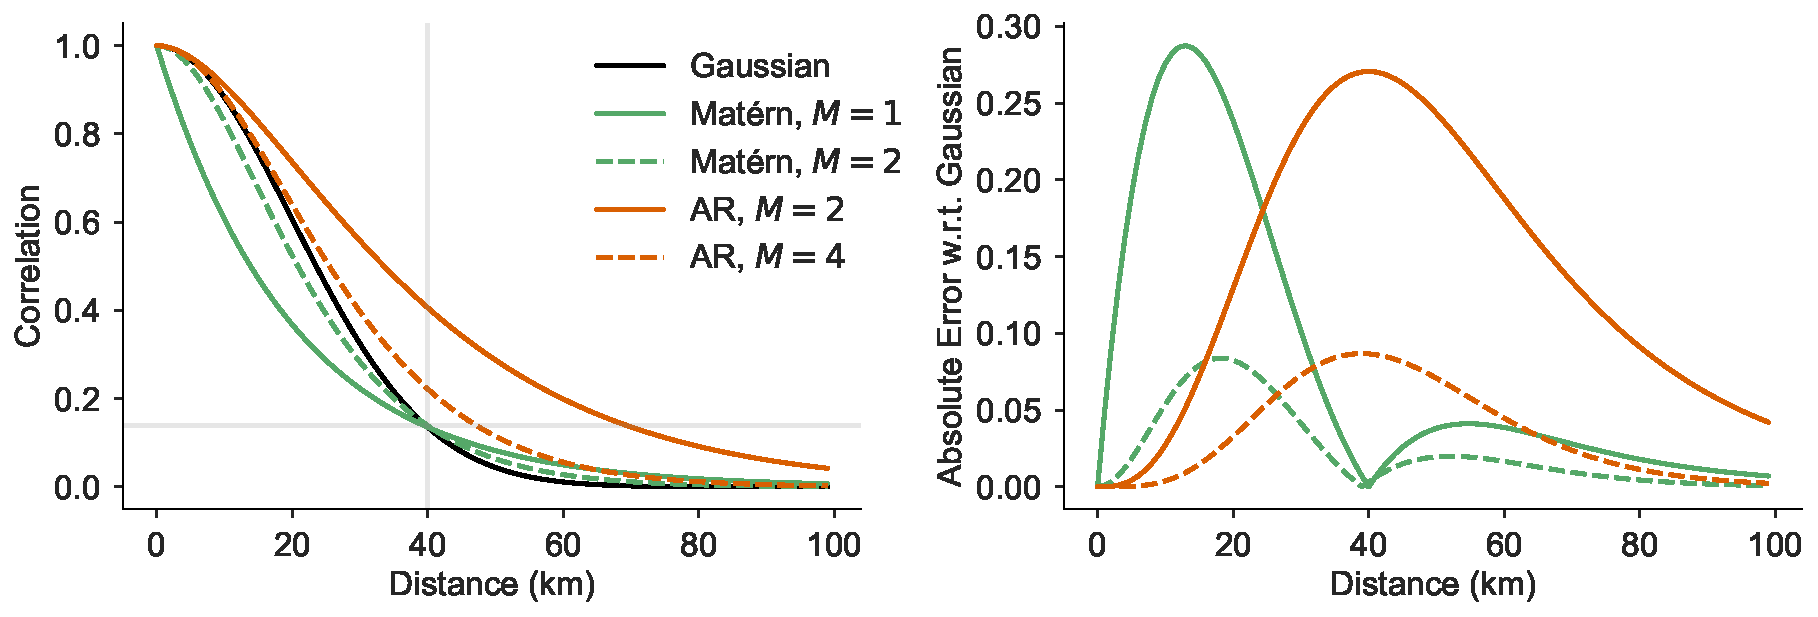
\includegraphics[width=\textwidth]{../figures/correlation_comparison.pdf}
    \caption{(a) Correlation as a function of distance given by
        Mat\'ern (green; \cref{eq:matern_corr_isostat}),
        auto-regressive (AR; orange),
        and Gaussian (black; $r_g(d) = \exp(-2 (d/4)^2)$) functions.
        For each, we choose a length scale of $\rangeh = 4$, noting for
        comparison purposes that this corresponds to $L=2$ using the notation in
        \citet{mirouze_representation_2010}.
        Finally, we note that we use $\ndims = 3$ to compute $\meandiff(M)$ (see
        \cref{eq:meandiff}) since this corresponds to our numerical experiments
        in \cref{sec:llc90}.
        (b) Absolute error considering the difference between the Mat\'ern and
        AR functions with respect to a Gaussian with the same length scale.
    }
    \label{fig:correlation_comparison}
\end{figure}

Additionally, \cref{fig:correlation_comparison}(b) shows the error in each
Mat\'ern and AR functions relative to a Gaussian.
We note that error for the Mat\'ern function is comparable to the AR function,
although $M$ is halved.
This has practical implications, since in both cases $M$ corresponds to the
number of inverse elliptic operator applications required for achieving a
correlation structure via the implicit diffusion approach (AR) or the approach
proposed here (Mat\'ern).
Thus, if the goal is to approximate a Gaussian, then using the direct Mat\'ern
shape results in half the required inverse elliptic solves.
However, we also stress that the desired shape of the correlation function will
be application dependent, and so we present a comparison from which
practitioners can take their pick.


\section{A Nonstationary and Anisotropic Mat\'ern Correlation Operator}
\label{sec:matern_operator}

Here we propose to use the SPDE operator described by \citet{RSSB:RSSB777}
as a means to describe an anisotropic, nonstationary correlation model in a
similar manner to the diffusion-based methods described in
\cref{ssec:wc01_review}.
To do so, we employ the ``mapping method'' described by \citet{RSSB:RSSB777}
which we show for the general $M$th order SPDE in \cref{ssec:mapping_method}.
In summary, the basic idea we present is to use the mapping method to
nondimensionalize or re-scale the elliptic operator.
We provide a simple scaling argument for why this is a good idea in
\cref{ssec:scaling_laplacian}, and discuss practical choices for the
nondimensionalization based on the grid scale in \cref{ssec:nonstationarity}.

\subsection{Mapping method or change of variables}
\label{ssec:mapping_method}

In \citet{RSSB:RSSB777} it is suggested that solving the SPDE in a transformed
coordinate system allows one to readily incorporate anisotropy and
nonstationarity into a Mat\'ern covariance model.
In this mapping method, we consider solutions to the isotropic, stationary SPDE
(\ref{eq:spde_iso}) to be defined in a transformed, or
``deformed'' \citep{sampson_nonparametric_1992}, space $\defdomain$.
Then, assume that we have a mapping $\defmap$ that maps between this transformed space
and our computational domain, $\domain$:
\begin{linenomath*}\begin{equation*}
    \defmap : \defdomain\ni\xh \rightarrow \x\in\domain \, .
\end{equation*}\end{linenomath*}
With this mapping, we can employ a change of variables
\citep{smith_change_1934} to rewrite the SPDE in the computational domain as:
\begin{linenomath*}\begin{equation*}
    \left(\dfrac{\deltah}{\defdet} -
    \nabla\cdot
    \dfrac{\defjac(\x)\defjac(\x)^T}{\defdet}
    \nabla\right)^M\uni(\x) =
    \defdet^{-1/2}\W(\x) \, .
\end{equation*}\end{linenomath*}
Here we have defined the Jacobian as
\begin{linenomath*}\begin{equation*}
    \defjac(\x_0) \coloneqq
    \dfrac{\partial \defmap}{\partial \xh}\Big|_{\defmap^{-1}(\x_{0})} \, ,
\end{equation*}\end{linenomath*}
and for now we assume that $\defmap^{-1}(\x_0)$ is well defined.
For our purposes, this turns out to be the case, but this becomes clear when
$\defjac$ is defined in \cref{ssec:scaling_laplacian}.
With the following definitions:
\begin{linenomath*}\begin{equation}
        K(\x) \coloneqq
        \dfrac{\defjac(\x)\defjac(\x)^T}{\defdet}
        \qquad
        \delta(\x) \coloneqq \dfrac{\deltah}{\defdet}
        \qquad
        \maternop \coloneqq \left(\delta(\x) - \nabla\cdot K(\x)\nabla\right)
    \label{eq:matern_definitions}
\end{equation}\end{linenomath*}
the SPDE in \cref{eq:spde_iso} can be written in the computational domain's coordinate system as
\begin{linenomath*}\begin{equation}
    \maternop^M \uni(\x) =
    \defdet^{-1/2}\W(\x) \, ,
    \label{eq:spde_general}
\end{equation}\end{linenomath*}
where zero flux, Neumann boundary conditions are applied at the boundaries
(see \cref{sec:discretization_matern} for details).
%We note as in \citet{RSSB:RSSB777} that this reproduces the deformation method
%introduced in \citet{sampson_nonparametric_1992}.

Here, we propose to use this generic form to define a square root of the
correlation matrix in a similar fashion to
\citet{weaver_correlation_2001, mirouze_representation_2010,
carrier_background-error_2010}
as follows,
\begin{linenomath*}\begin{equation}
    \corrMat^{1/2} \coloneqq \normalizer
    \maternop^{-M}
    \defdet^{-1/2} \, ,
    \label{eq:matern_operator}
\end{equation}\end{linenomath*}
where $\normalizer$ is
once again a variance-preserving normalization matrix defined by the operations
that precede it.
In this model,
anisotropy and nonstationarity are controlled by
$\defjac(\x)$, and in the following sections
we discuss how this can be assigned for
practical applications in geophysical inverse problems.
We note that in this discussion we loosely mix the use of
finite dimensional matrices and infinite dimensional operators
in order to ease the presentation, but we provide a more careful
derivation of their discretized forms relevant to our numerical experiments in
\cref{sec:discretization_matern}.

\subsection{Scaling the Laplacian term for anisotropy}
\label{ssec:scaling_laplacian}

Here we focus on parameterizing $\defjac(\x)$ in order to achieve an anisotropic
correlation model that is relevant for variational data assimilation.
We illustrate our choice with a scaling argument focusing on how $K(\x)$
influences correlation length scales.

Consider a 3D field $\uni(\x)\sim U$ that exhibits spatial variability at the
length scales, $L_x$, $L_y$, and $L_z$ in the direction of longitude, latitude,
and height, respectively,
where $L_x$, $L_y$ $>>$ $L_z$, such that the field exhibits highly
anisotropic fluctuations.
This is a common situation in large scale geophysical fluid
dynamics, where fields (e.g.\ temperature, velocity) exhibit length scales of
variability that are much greater in either horizontal dimension compared to the
vertical \citep[e.g.][]{vallis2006}.
%\footnote{
%    We make a note on the terminology used here.
%    In oceanography, the difference in horizontal and vertical scales
%    is a result of the small aspect ratio, or the shallow fluid nature of the ocean.
%    Because of the vast difference in scales, the horizontal dimensions are
%    sometimes considered entirely independent of the vertical, and ``anisotropy''
%    can be used to refer to heterogeneity between the horizontal components.
%    However, here we use anisotropy to refer to the difference between horizontal
%    and vertical scales, resulting from the small aspect ratio \citep{vallis2006}.
%}
Without any rescaling, i.e.\ without $K$,
the Laplacian term in $\maternop$ is unbalanced
\begin{linenomath*}\begin{equation}
    \begin{aligned}
        \nabla^2 \uni(\x)
            & \sim \dfrac{U}{L_x^2} + \dfrac{U}{L_y^2} + \dfrac{U}{L_z^2} \\
            & \simeq \dfrac{U}{L_z^2} \, .
    \end{aligned}
    \label{eq:iso_lap}
\end{equation}\end{linenomath*}
As a result, the correlation model will
have unrealistically large (small) correlations in the vertical (horizontal).
Our goal is therefore to define the elements of $K$ such that each term is of
the same order of magnitude.
%and
%\begin{linenomath*}\begin{equation*}
%    \nabla\cdot K\nabla \sim 3U \, .
%\end{equation*}\end{linenomath*}

To achieve this balance between Laplacian terms, we suggest a straightforward,
perhaps obvious, specification of $\defjac$:
\begin{linenomath*}\begin{equation*}
    \defjac =
        \begin{pmatrix}
            L_x & 0 & 0     \\
            0 & L_y & 0     \\
            0 & 0   & L_z   \\
        \end{pmatrix} \, ,
\end{equation*}\end{linenomath*}
where we simply ignore the off-diagonal elements of $\defjac$.
The determinant in this case is $\defdetnox = L_xL_yL_z$ and
according to the definitions in \cref{eq:matern_definitions}:
\begin{linenomath*}\begin{equation*}
    K =
        \begin{pmatrix}
            1/L_z & 0 & 0     \\
            0 & 1/L_z & 0     \\
            0 & 0   & L_z/(L_xL_y)   \\
        \end{pmatrix} \, ,
\end{equation*}\end{linenomath*}
so that
\begin{linenomath*}\begin{equation*}
    \nabla\cdot K\nabla\uni(\x) \sim \dfrac{3}{L_xL_yL_z}U \, .
\end{equation*}\end{linenomath*}
The key is that $K$ scales each term in the Laplacian so that they are
approximately the same order of magnitude, and the operator is balanced in all
directions.
In the case of nonstationarity, we simply require this balance to apply locally
and allow the length scales $L_x$, $L_y$, and $L_z$ to vary in space.
%This example can further be extended by allowing the length scales $L_1$ and
%$L_2$ to vary in space, such that correlations are nonstationary.


\subsection{Harnessing the grid scale for nonstationarity}
\label{ssec:nonstationarity}

At this point, we must prescribe values for the normalizing length scales
$L_x(\x)$, $L_y(\x)$, and $L_z(\x)$ in order to fill $\defjac(\x)$.
Considering the scaling analysis of the Laplacian in
\cref{ssec:scaling_laplacian}, a simple yet reliable choice for these
is to use the underlying grid-scale of the numerical model (e.g.\ the ocean or
atmosphere general circulation model).

We consider using the length scale of the grid elements to be reasonable
because a baseline level anisotropy and nonstationarity is usually encoded
into the grid.
A prime example of this nonstationarity is represented by the vertical axis of
ocean model grids, which are designed to capture a variety of behavior in a
computationally efficient manner \citep{griffies_fundamentals_2004}.
Toward the surface, the ocean is tightly coupled to the atmosphere, sea ice, and
rivers, and ocean models use a finely resolved vertical grid to capture the
ocean component of these coupled processes.
In the interior ocean, well below the mixed layer, the ocean acts more like stacked layers, and
variation in properties like temperature and salinity occurs over much larger
distances than at the surface \citep{talley_descriptive_2011}.
Vertical grids are correspondingly much coarser.
As a concrete example, the height-based vertical grid we use in \cref{sec:llc90}
varies from $\sim 5-10$~m near the surface, and spacing increases to
$\bigo(100)$~m below 1,000~m (\cref{fig:llc90_correlation_maps}(c)).
By using the grid elements directly, our correlation model can capture the
nonstationarity motivated by the physical processes which influence the model
grid's development.

Another justification for using the grid elements to specify $\defjac(\x)$ is
that this provides a practical and intuitive nondimensionalization.
With this definition, the correlation model exhibits isotropic and stationary
behavior within the nondimensional space defined by the computational grid.
As such, the idealized correlation function (\cref{eq:matern_corr_isostat})
applies relative to the grid spacing, and one can view $\rangeh$ as an
intuitive, nondimensional parameter controlling the
``number of neighboring grid cells'' at which correlation decays to 0.14.
Our numerical experiments in \cref{sec:llc90} show that this is a good
approximation in the case of a realistic global ocean model grid.


\section{Application to the Global Ocean}
\label{sec:llc90}

Here we show results from a numerical implementation of the correlation model
described in \cref{sec:matern_operator}.
For this application we use the ``Lat-Lon-Cap'' (LLC) grid used by the ECCOv4
state estimate \cite[][see Sec. 2 for a complete description of the grid]{forgetECCOv4}.
The overall goal with these numerical experiments is to show that even in this
relatively complicated global grid, the
correlation model generally follows the expected Mat\'ern correlation structure
(\cref{ssec:llc90_correlations}), while maintaining
anisotropy and nonstationarity that is relevant to the physical system
(\cref{ssec:llc90_correlation_maps}).
Additionally, we show how Neumann boundary conditions to the differential
operator affect the solution in \cref{ssec:llc90_boundary_effects}.
We finish
by showing that the model can be applied efficiently with a relatively imprecise
solver tolerance (\cref{ssec:tolerance}) and that it is relatively cheap even
when the number of applications, $M$, is greater than one
(\cref{ssec:iters_and_apps}).

For all experiments, we compute statistical quantities from 1,000 samples using
the block-Successive Over Relaxation (SOR) method which is described fully in
\cref{sec:block_sor}.
Additionally, we use
$L_x(i,j) = \Delta x_g(i,j)$, $L_y(i,j) = \Delta y_g(i,j)$,
and $L_z(k) = \Delta r_f(k)$ (\cref{fig:mitgcm_grid}) where we have switched
from the spatial coordinate $\x\in\domain$ to the computational grid indices $i$, $j$, $k$.
All experiments are performed with a 3D field, which could represent an ocean
state property like temperature or salinity.

\subsection{Correspondence with theoretical correlation structure}
\label{ssec:llc90_correlations}

We first show that the sample correlation structure computed on the LLC
grid corresponds with the analytical expression for
Mat\'ern-type correlations.
For this comparison we compute the correlation field in the transformed space
$\defdomain$, where the random field can be considered isotropic and stationary.
Because we use the grid spacing to define this mapping, the correlation
distances are computed simply by counting the number of neighboring grid cells in each
direction from the point in consideration.
%We refer to this distance as $\delta\hat{x}$, $\delta\hat{y}$, and
%$\delta\hat{z}$ for the longitudinal, meridional, and vertical dimensions
%respectively.

\cref{fig:llc90_correlations} shows the comparison between the theoretically
expected correlation structure (black) and the numerically computed sample
correlation structure for
$\rangeh = \{5, 10, 15, 20\}$ (color) using $M =\{1,2,4,8\}$ (panels).
The correlation is computed in the direction of longitude, indicated by
$\delta i$.
The shading indicates the spread between the first and ninth deciles of the
sample correlation, computed at all depth levels and latitudes from
70$^\circ$S to 37$^\circ$N at 127.5$^\circ$W - a subset chosen simply to ease the
calculation.
Similar plots showing correlation in the meridional and vertical directions are
shown in the Supplemental Material.

Generally speaking, the colored curves match the analytical expression well, and
each colored curve intersects the horizontal gray line, indicating a correlation
value of 0.14, where $\rangeh = \delta i$.
We note that the largest spread in the computed correlation structure occurs
when $M=1$, especially for larger values of $\rangeh$.
Considering an analogy to Laplacian versus biharmonic damping in ocean models
\citep[e.g.][]{holland_role_1978,griffies_biharmonic_2000}, we suggest that
there is more spread when $M=1$ because the operator $\maternop^{-1}$
contains a only a Laplacian term.
Compared to the cases when $M>1$, which contain biharmonic and higher order
Laplacian terms in $\maternop^{-M}$, the Laplacian case is less
scale-selective.
That is, the operator does not cutoff higher frequency variability sharply,
allowing noise to pollute the sample statistics \citep[see][Section 2 for a quantitative
description of this cutoff in frequency space]{griffies_biharmonic_2000}.
We note, however, that the spread still allows for a reasonable interpretation
that the operator $\maternop^{-1}$ captures the behavior of the analytical Mat\'ern correlation
function.

\begin{figure}
    \centering
    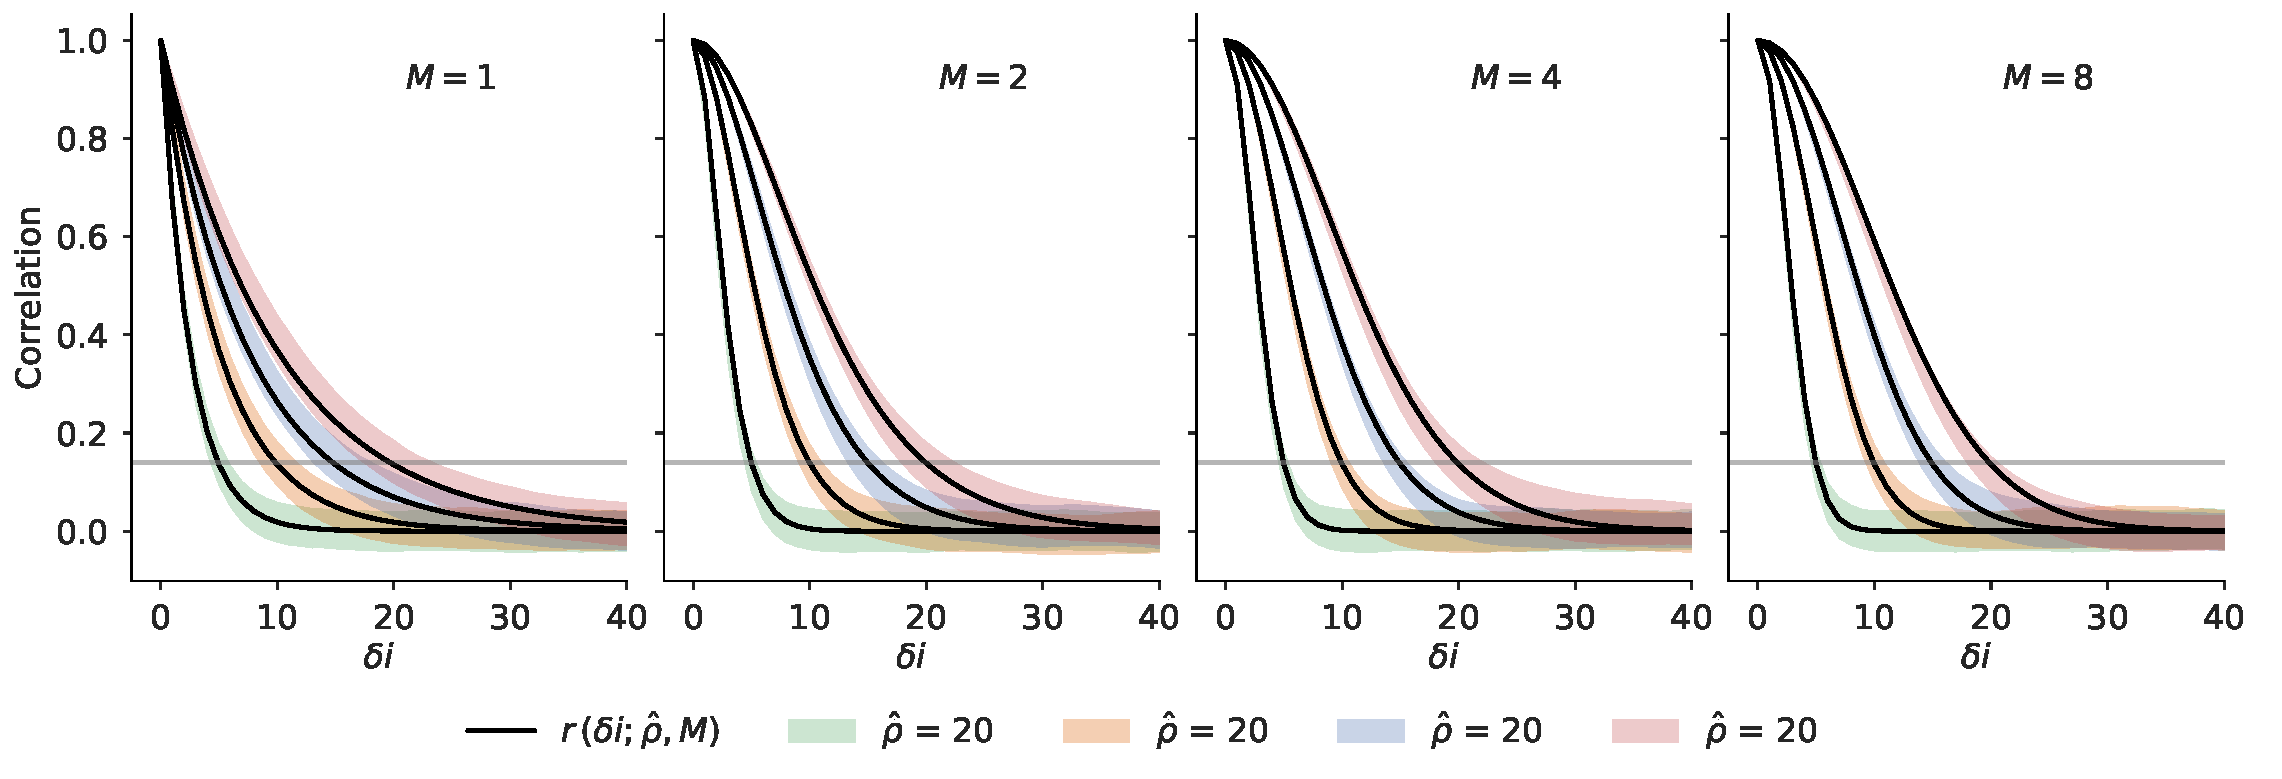
\includegraphics[width=\textwidth]{../figures/matern_llc90_correlation_theory_vs_m_ix.pdf}
    \caption{Correlation structure computed from the theoretical Mat\'ern
        correlation function (black; \cref{eq:matern_corr_isostat}) and from
        1,000 samples using a subset of the ``Lat-Lon-Cap'' grid within the
        Pacific Ocean (shaded coloring).
        The sample correlation is computed in the zonal direction, $\delta i$,
        indicating number of neighboring grid cells from
        127.5$^\circ$W.
        The shading indicates the spread between the first and ninth deciles,
        based on sample correlations at all depth levels and latitudes from
        70$^\circ$S and 37$^\circ$N.
        Similar plots showing correlation as a function of meridional and
        vertical distance are provided in the Supplemental Material.
        Correlation is computed from 1,000 random samples with a tolerance of
        $10^{-3}$ (see \cref{ssec:tolerance}).
    }
    \label{fig:llc90_correlations}
\end{figure}

\subsection{Sample correlation maps}
\label{ssec:llc90_correlation_maps}

Maps of the sample correlation field at two locations on the LLC
grid are shown in
\cref{fig:llc90_correlation_maps}.
For these calculations we use a perhaps unrealistically large correlation length scale
defined by $\rangeh=20$ for illustrative purposes.
First, we compare panels (a) and (b) of \cref{fig:llc90_correlation_maps}, which
show the sample correlation computed at
(0.2$^\circ$N, 127.5$^\circ$W, 722~m depth) and
(10.5$^\circ$N, 87.5$^\circ$W, 5~m depth), respectively.
In panel (a), the correlation structure is anisotropic such that the field is
ellipsoidal, with correlation length scales that are
relatively longer zonally than meridionally.
On the other hand, the correlation structure shown in panel (b) is closer to
being isotropic, qualitatively speaking, since the field is relatively circular
except where it intersects with the coast.

In this example we obtain longer correlation length scales at the equator
because the LLC grid is defined with smaller meridional grid spacing here in
order to resolve tropical, zonal currents;
see \cref{fig:llc90_correlation_maps}(c) for a comparison of $\Delta x $ and
$\Delta y$ near the equator.
To clarify why this corresponds to the correlation structure we obtain,
consider the normalization of the Laplacian discussed in
\cref{ssec:scaling_laplacian}, and the interpretation of $\rangeh$ described
in \cref{ssec:llc90_correlations}.
Since the meridional grid refines near the equator, the number of grid cells at
which correlation drops to 0.14 covers a shorter distance meridionally compared
to the zonal direction.

\begin{figure}
    \centering
    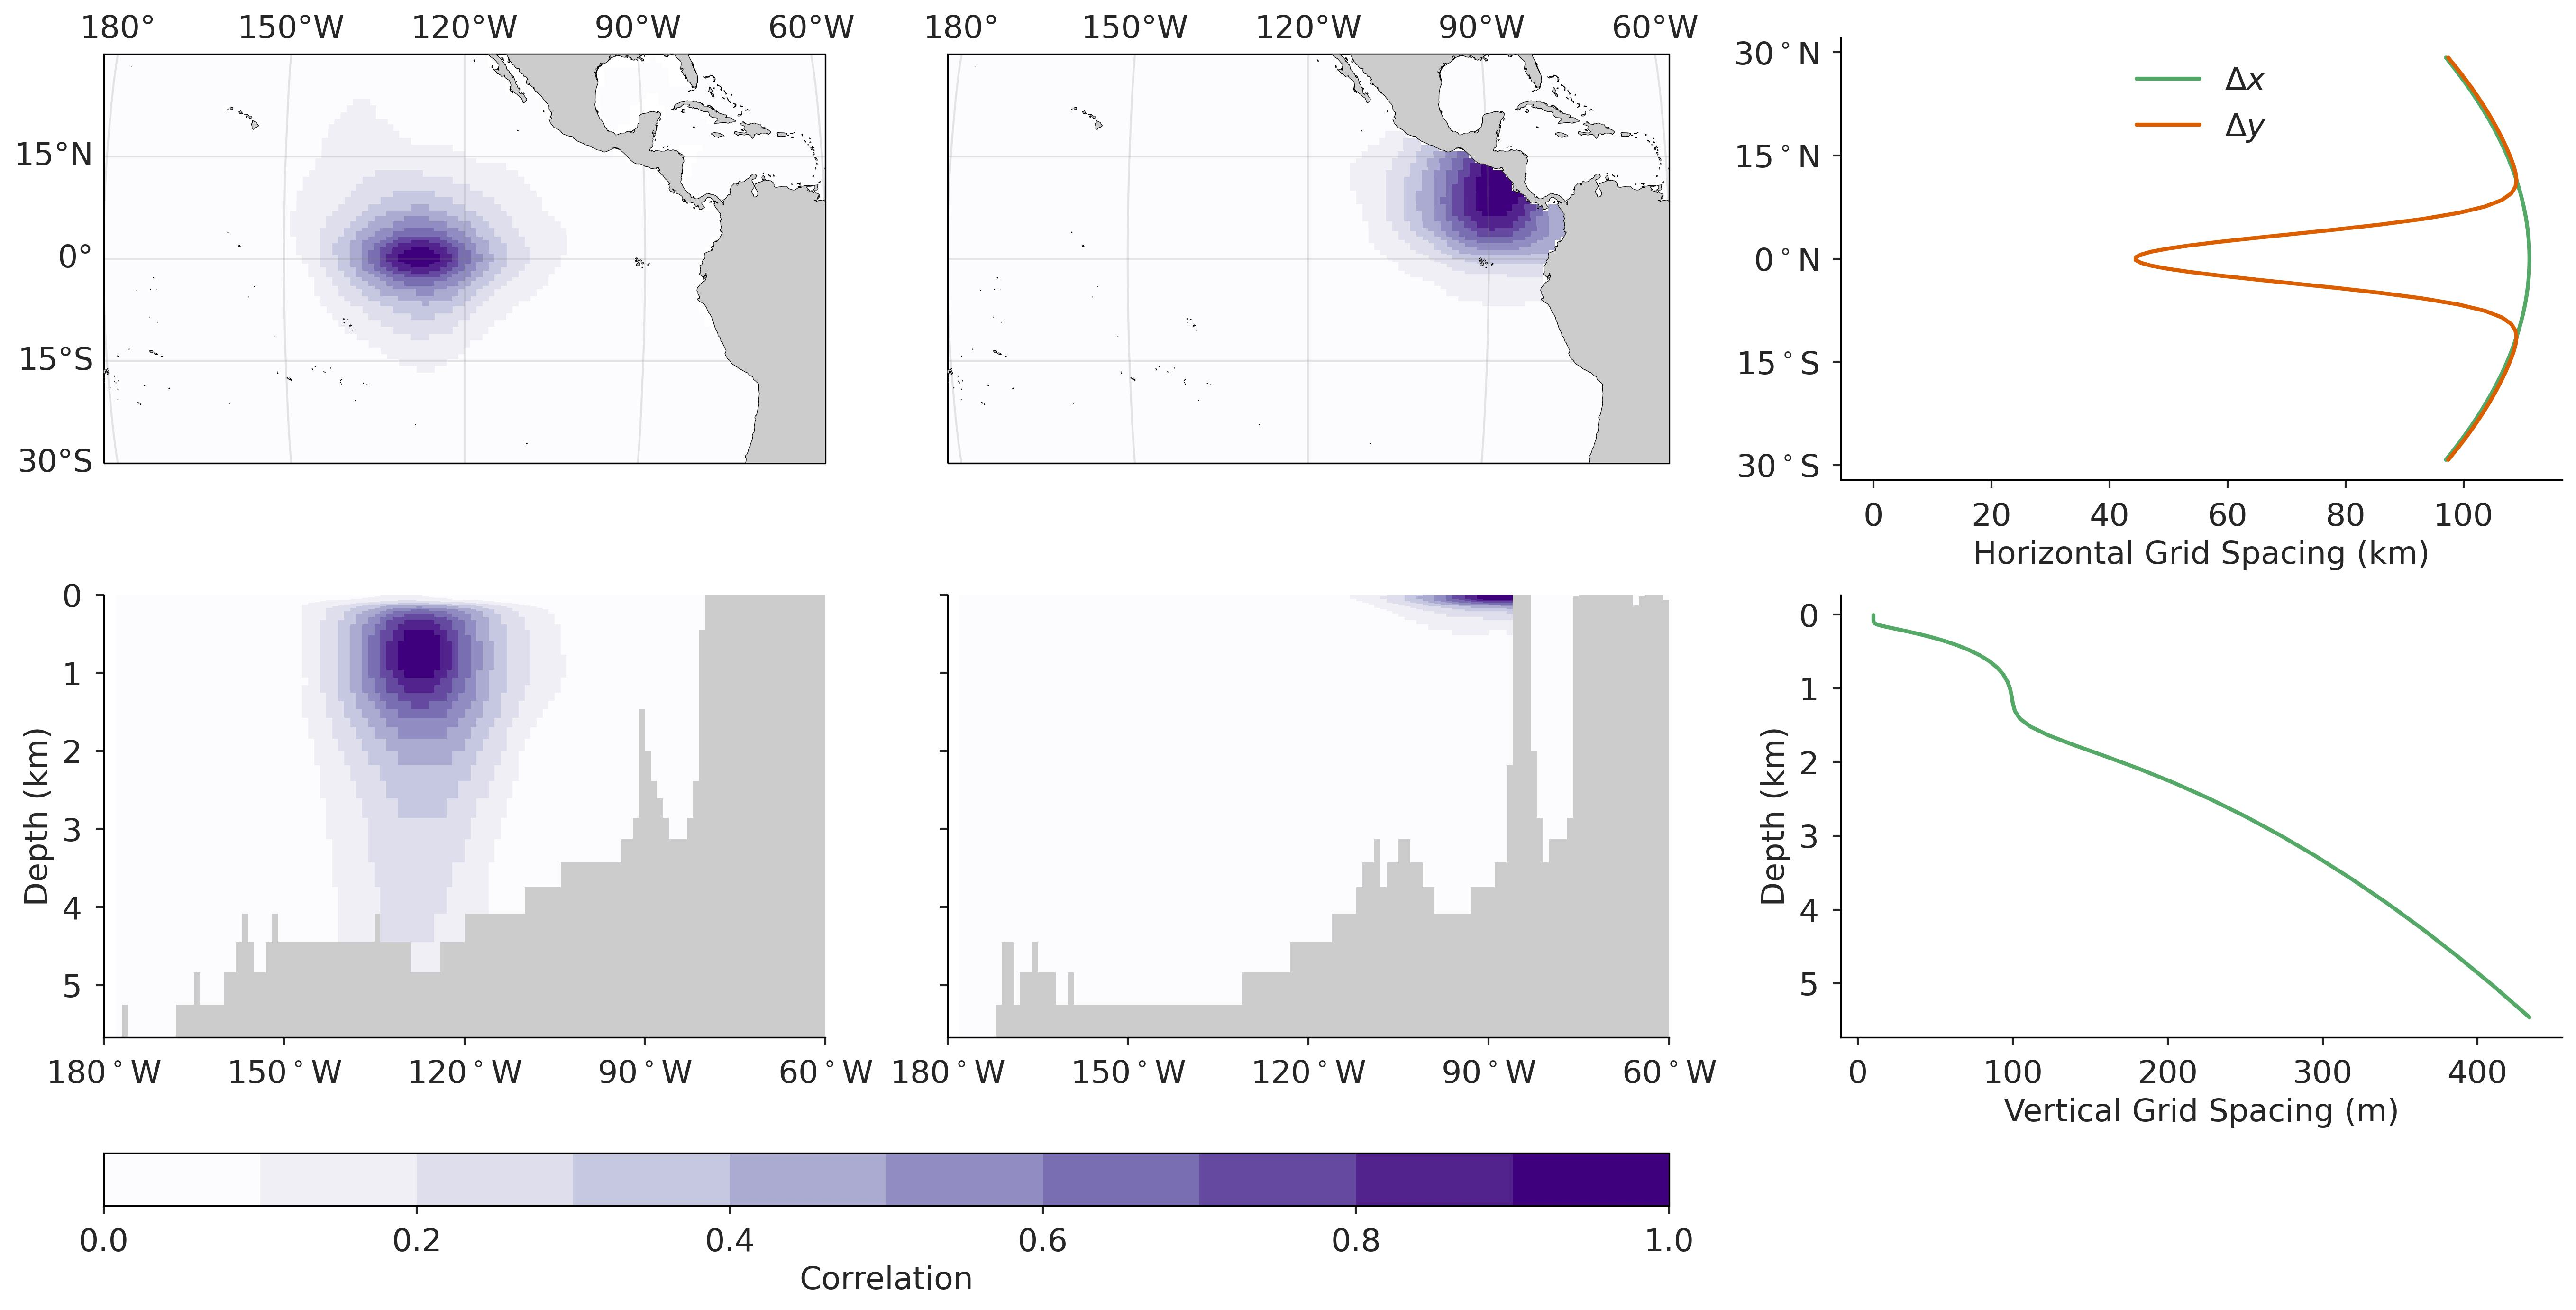
\includegraphics[width=\textwidth]{../figures/huge_correlation_map_02apps.jpg}
    \caption{Two sample correlation fields and a depiction of the computational
        grid.
        (a \& b) Sample correlation field in the latitude-longitude plane at
        (0.2$^\circ$N, 127.5$^\circ$W, 722~m depth) and
        (10.5$^\circ$N, 87.5$^\circ$W, 5~m depth), respectively.
        (c \& d) The same sample correlation fields as above, shown in the
        depth-longitude plane.
        (e \& f) The local horizontal and vertical grid spacing, respectively.
        The correlation fields are computed from 1,000 random samples,
        with $\rangeh = 20$, $M=2$, and a solver tolerance of $10^{-3}$ (see
        \cref{ssec:tolerance}).
    }
    \label{fig:llc90_correlation_maps}
\end{figure}

Panels (d) and (e) of \cref{fig:llc90_correlation_maps} show the extent of the
sample correlation fields from (a) and (b) in depth-longitude space, respectively.
In panel (d) the correlation remains greater than 0.1 until roughly 4-km
depth, whereas the correlation structure in panel (e) is much more confined to
the surface.
Once again, the difference in behavior is due to the fact that the vertical grid
spacing is smaller toward the surface than it is below 1000~m in order to
resolve the ocean mixed layer and surface processes, see
\cref{fig:llc90_correlation_maps}(f).

\subsection{Pointwise sample standard deviation}
\label{ssec:llc90_boundary_effects}


The pointwise, sample standard deviation is shown in \cref{fig:std_ratio}, where
it is represented as a ratio with respect to the ``expected'' value from
\cref{eq:matern_variance} for an isotropic, stationary Mat\'ern field.
Throughout most of the domain, the sample standard deviation is approximately
equal to the theoretical value.
Near continental boundaries the standard deviation is inflated, especially
for large values of $\rangeh$ and in regions of tightly confined topographic
boundaries such as in the Caribbean Sea.
This deviation near the boundaries is expected for correlation models based on
the solution of differential equations
\citep[e.g.][]{weaver_correlation_2001,RSSB:RSSB777}, as a result of the zero
flux, Neumann boundary conditions used to find the solution.
Thus, it is necessary to estimate the sample variance to normalize the
covariance model (i.e.\ formulate the diagonal entries of $\normalizer$,
\cref{eq:matern_operator}), rather than use the theoretical value directly.
Throughout this work, we have used the sample estimates shown in
\cref{fig:std_ratio} to obtain correlation fields.
Given the correspondence to theoretical correlation structure in
\cref{ssec:llc90_correlations}, this appears to be reliable.
Other methods to remove boundary effects, for instance through the
combination of Neumann and Dirichlet boundary conditions as shown for the
implicit diffusion approach in Section 4.2 of
\citet{mirouze_representation_2010}, could be explored in future work.

\begin{figure}
    \centering
    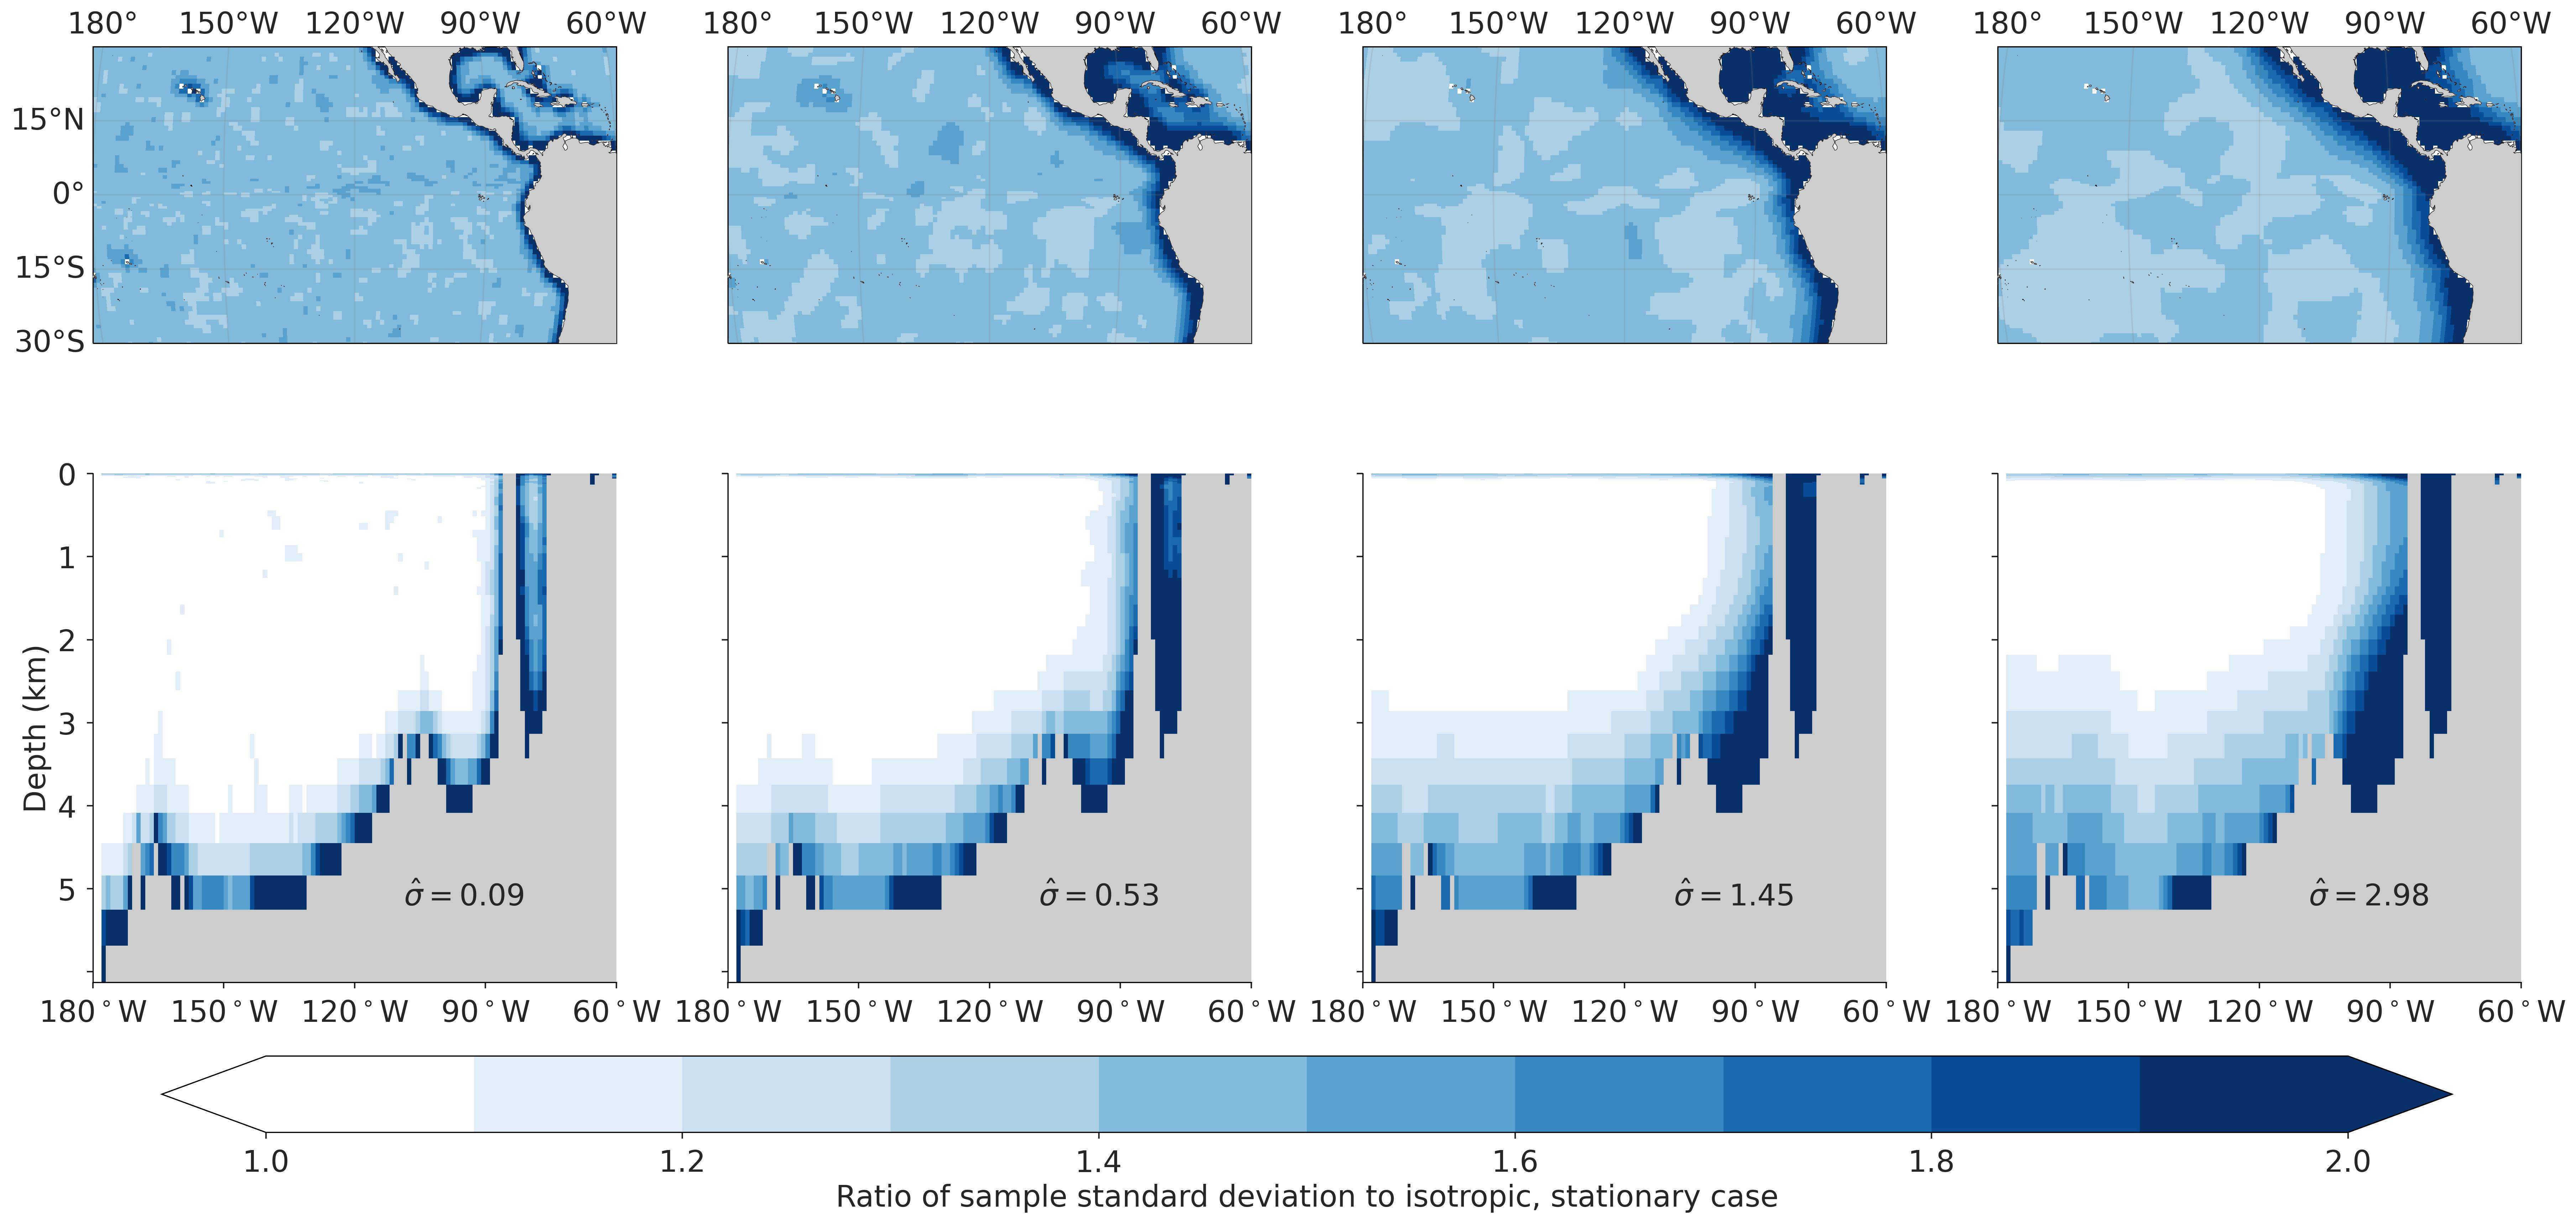
\includegraphics[width=\textwidth]{../figures/std_ratio_02apps.jpg}
    \caption{The ratio of the sample standard deviation to the value computed
        from \cref{eq:matern_variance} for an isotropic, stationary Mat\'ern
        field. Panels (a-d) show the ratio in the latitude-longitude plane at
        the surface for $\rangeh=\{5,10,15,20\}$, respectively. Panels (e-h)
        show the corresponding fields in the depth-longitude plane along 10.5$^\circ$N.
        The largest deviations from the theoretical value are near the boundaries, as
        expected.
        All fields are estimated from 1,000 random samples using $M=2$ and a
        solver tolerance of $10^{-3}$ (see \cref{ssec:tolerance}).
    }
    \label{fig:std_ratio}
\end{figure}

\subsection{High efficiency with low precision}
\label{ssec:tolerance}

The numerical results shown in this section have employed the
iterative algorithm in \cref{sec:block_sor} to obtain approximate correlation
statistics.
As with any iterative algorithm, one must specify a
tolerance that can be used to determine when the algorithm has converged to an
approximate solution.
Within this framework, one can always set a tolerance based on the numerical
precision being used to be confident that the solver has converged.
However, in this section we show that this is likely to be
unnecessarily ambitious.

To be specific, \cref{fig:error_and_iters}(a) shows the relative error in the
approximation that correlation is equal to 0.14 when $\rangeh = \delta i$
for $\rangeh = \{5, 10, 15, 20\}$ (i.e.\ corresponding to the curves in
\cref{fig:llc90_correlations}).
The error in the approximation is shown for a range of solver tolerances,
where $10^{-15}$ is chosen as an approximate lower bound tolerance for double
precision.
For tolerances at $10^{-3}$ and smaller, the error coverges to roughly the same
value, indicating that the desired statistics of the correlation
model are obtained even with a relatively imprecise solve.
We note that \citet{carrier_background-error_2010} describe similar findings
with the implicit diffusion correlation model.

The motivation for using a high tolerance is indicated by
\cref{fig:error_and_iters}(b), which shows how the number of iterations required
to converge increases with the specified tolerance.
Solving to a tolerance of $10^{-15}$ requires a factor of 6-13
more iterations than are required with a tolerance of $10^{-3}$.
Of course, the specific computational savings obtained will depend on the
iterative method that is being used, but we provide this as a concrete example
to highlight that an imprecise solve is both valid and advantageous.

\begin{figure}
    \centering
    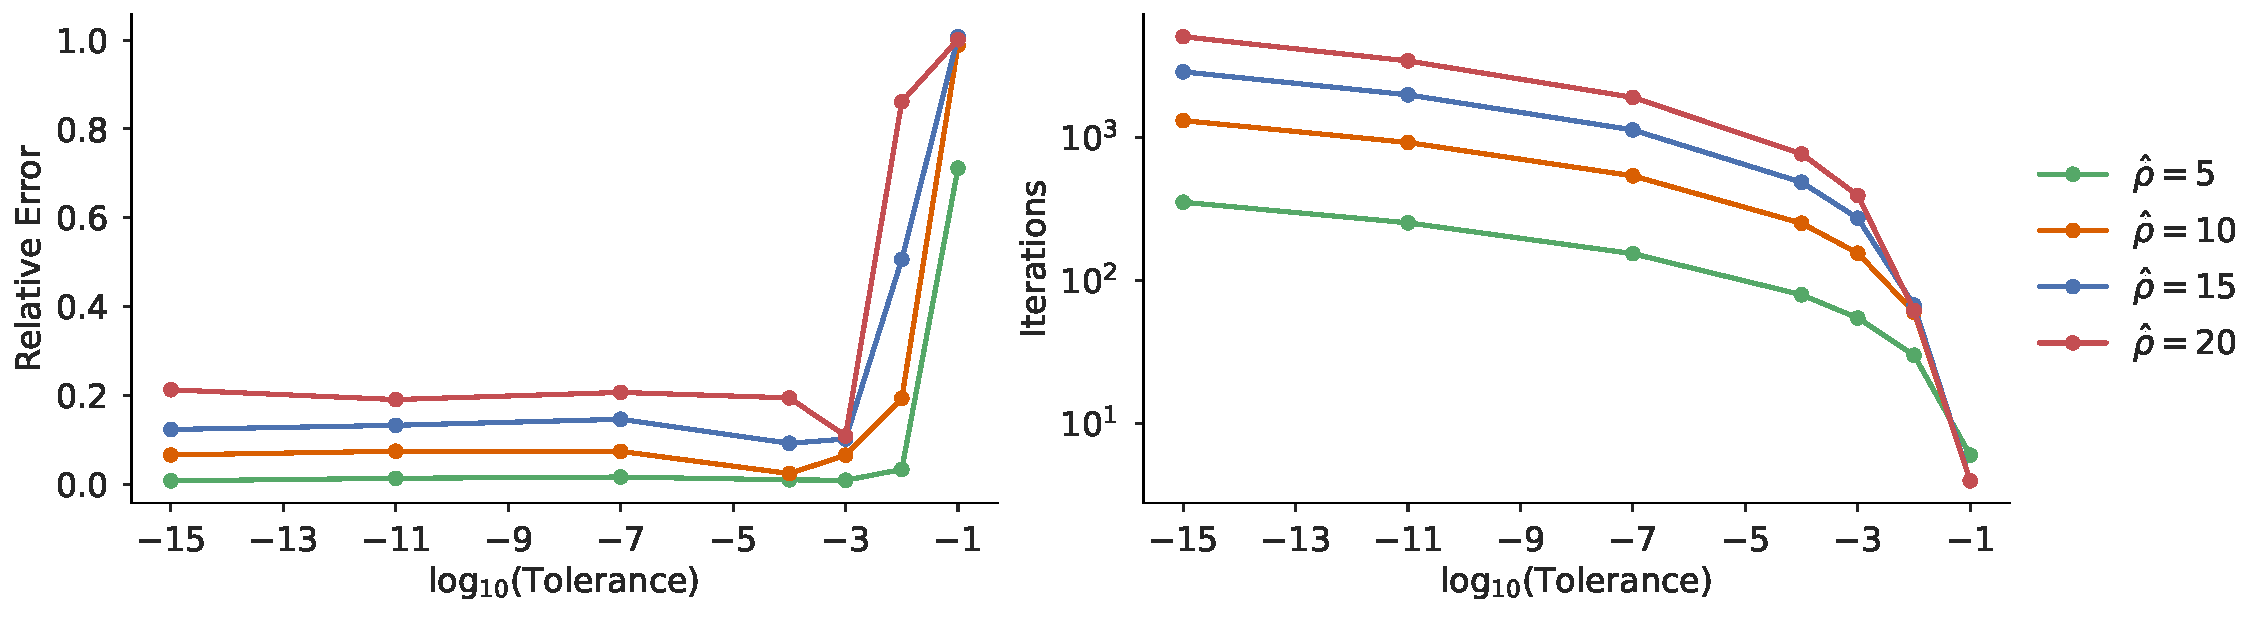
\includegraphics[width=\textwidth]{../figures/matern_llc90_error_and_iters_01apps.pdf}
    \caption{(a) The relative error in the approximation that correlation equals
        0.14 when $\rangeh=\delta i$, as a function of the tolerance used
        for the iterative block-SOR method described in \cref{sec:block_sor}.
        Each curve is computed as the error between the theoretical (black)
        curve and the average of each shaded curve shown in \cref{fig:llc90_correlations}.
        (b) The number of iterations required for the block-SOR method to
        converge to the specified tolerance.
        Averages are computed from 1,000 samples using $M=1$.
    }
    \label{fig:error_and_iters}
\end{figure}

\subsection{Rapid convergence for $M>1$}
\label{ssec:iters_and_apps}

For applications where a Gaussian correlation structure is desired, the
correlation model presented here requires $M>1$ to approach the Gaussian
structure (\cref{fig:correlation_comparison}).
Moreover, it could also be desirable to use $\maternop^{-M}$ with $M>1$,
given that $M=1$ produces larger spread in the correlation structure
(\cref{fig:llc90_correlations}(a)), and because the correlation structure drops
off much more rapidly for neighboring points.
For these cases, it may be natural to assume that using this model with $M>1$
would be less efficient than when $M=1$ because it requires multiple
applications of an inverse elliptic operator.
However, here we show that this is evidently not necessarily true and it is
actually often \textit{more} efficient to use $M>1$ than $M=1$.

\cref{fig:iters_and_apps}(a) shows the total number of iterations required to
find a solution to \cref{eq:matern_operator}, for a variety of combinations of
$\rangeh$ and $M$.
Here, ``total iterations'' refers to all block-SOR iterations
required by the algorithm in \cref{sec:block_sor}, summing over all applications
of $\maternop^{-M}$.
Evidently, using $M>1$ actually requires \textit{fewer} total iterations to converge to a
solution than when $M=1$.
The reason for this is as follows.
For any value of $\rangeh$, $\deltah$ increases linearly with $M$, which
increases the amplitude of the diagonal elements of the matrix representation of
$\maternop$.
In each case, the off-diagonal matrix elements, determined by the Laplacian
operator, remain fixed.
Thus, the matrix becomes more diagonally dominant:
the amplitude of the diagonal elements increases relative to the sum total of
off-diagonals.
The degree of diagonal dominance is an important property for
determining the convergence of our SOR-based elliptic solver, where a more
diagonally dominant matrix tends to converge faster \citep{golub_matrix_2013}.
Evidence of this behavior can be seen in \cref{fig:iters_and_apps}(b), which shows the
number of iterations required for each individual application of
$\maternop^{-1}$ to converge.
Here we see that each application gets cheaper as $M$, and therefore $\deltah$,
increases and the improvement per iteration is evidently enough to reduce the total
iterations, shown in panel (a).
The exception to this behavior is when $\rangeh = 5$, where for $M\ge 4$
the total number of iterations overtakes the case of $M=1$ due to the repeated
solves.

\begin{figure}
    \centering
    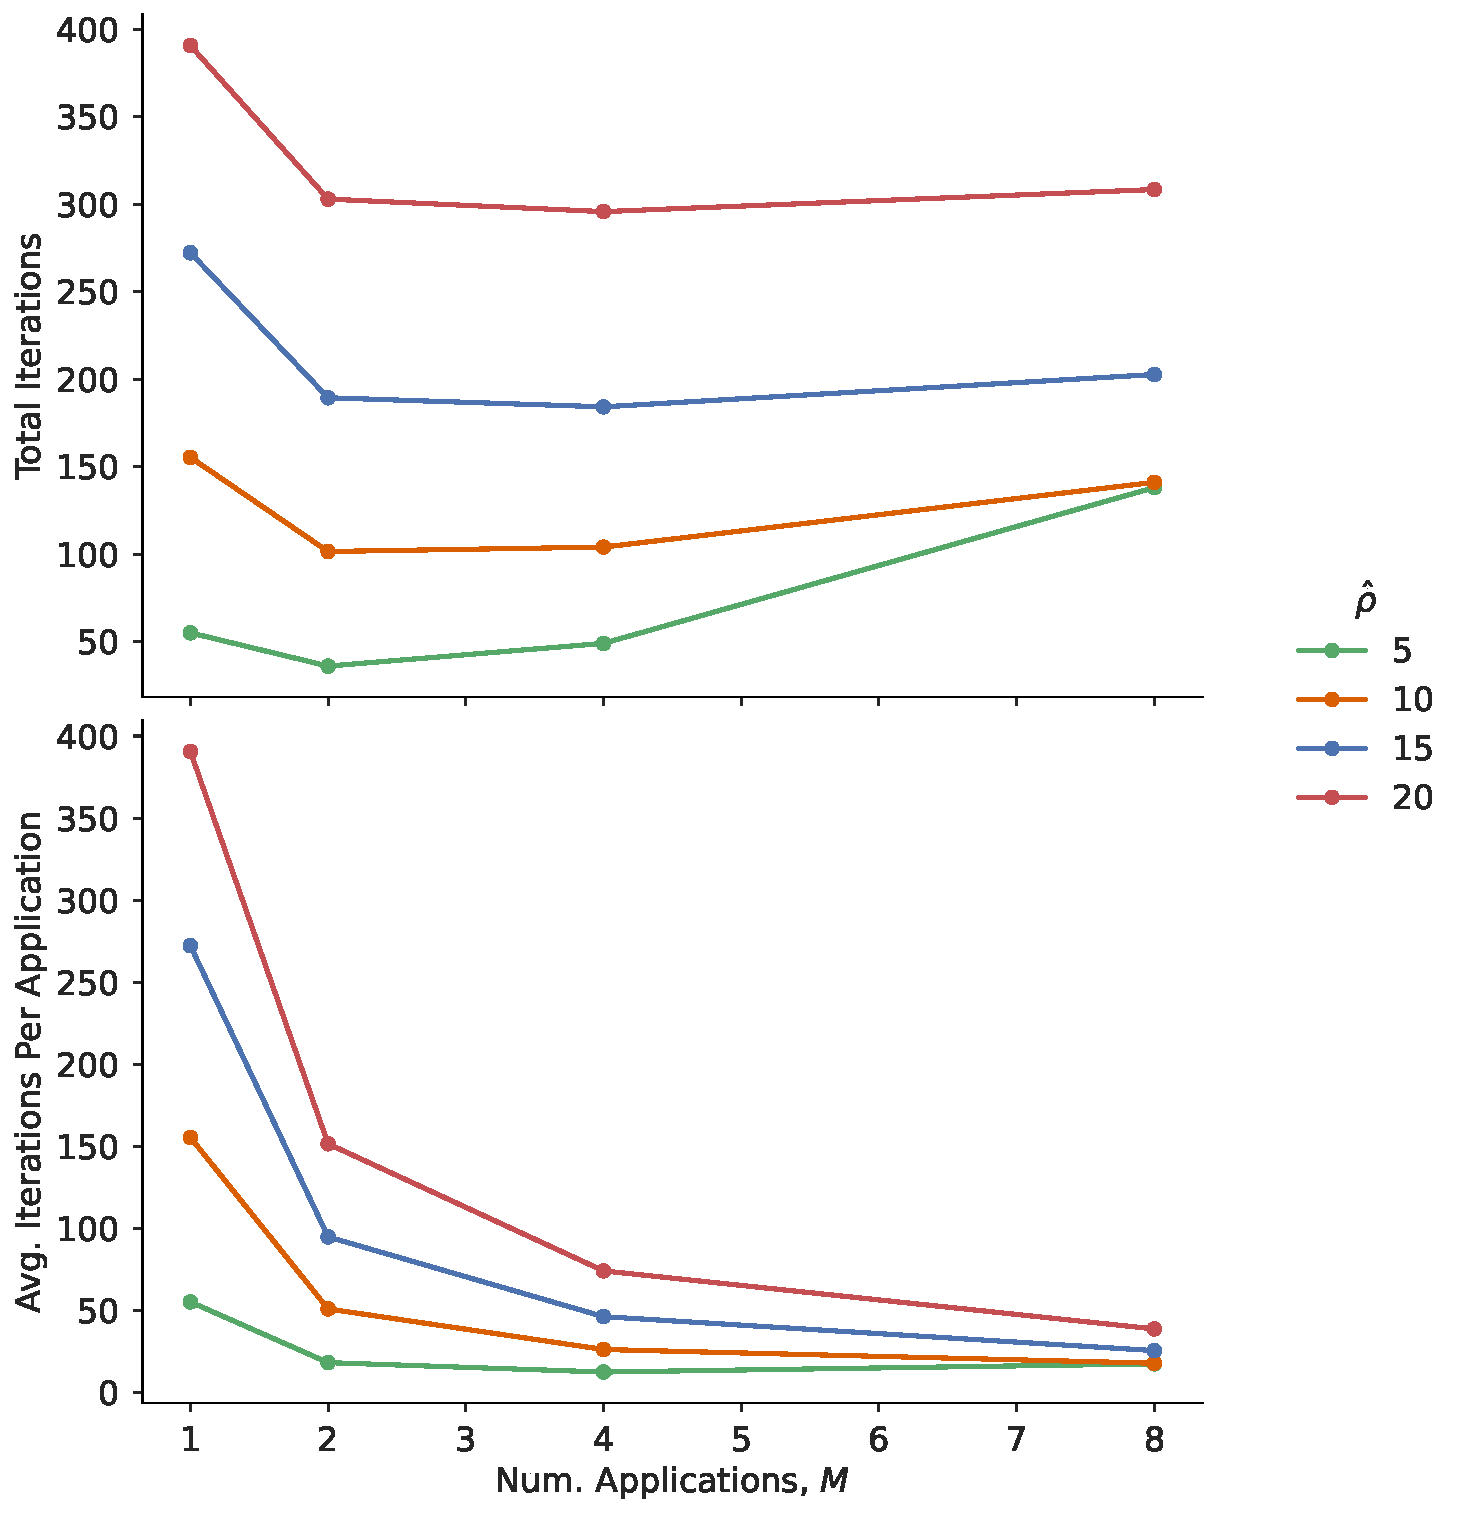
\includegraphics[width=.7\textwidth]{../figures/iterations_vs_applications.pdf}
    \caption{(a) Total number of iterations required to compute
        $\unis = \maternop^{-M}\mathbf{z}$, for a standard normally distributed
        vector $\mathbf{z}\in\ndspace$.
        ``Total iterations'' is represented as the average number of total
        iterations from 1,000 random samples.
        (b) The average number of iterations per application of
        $\maternop^{-M}$, as a function of $M$.
        For all $\rangeh$ and $M$ combinations, each application gets cheaper as
        $M$ increases.
        To compute the ``average iterations per application'', we take the
        average iteration per application of $\maternop^{-M}$, and compute the sample
        average of this quantity from 1,000 random samples.
        Solver tolerance is set to $10^{-3}$.
    }
    \label{fig:iters_and_apps}
\end{figure}


\section{Discussion}
\label{sec:matern_discussion}

In this work we have shown a general methodology which can be used to achieve
nonstationary and anisotropic Mat\'ern type correlation structures within a
domain with complex boundaries.
To summarize, the general procedure is as follows.
First, one chooses a normalization length scale for each dimension, thereby
defining (the Jacobian of) a mapping between a space where correlation is
isotropic and stationary, and the more complex domain.
These normalizing length scales are essential because they determine the local
anisotropy and nonstationarity of the correlation operator.
Next, one must choose a range parameter, determining the distance relative to
the normalizing length scales at which correlation drops to 0.14.
Finally, one selects the shape of the correlation structure, which also sets the
number of times the elliptic PDE must be solved.

Our presentation has focused on the practical application of this
correlation operator within an ocean general circulation model.
As such, we set the normalizing length scales based on the local grid
scale.
With this setting, the range parameter is shown to be a highly intuitive dial,
controlling correlation length scales as a simple function of the number of
neighboring grid cells.
Using this definition was further shown to be beneficial at the equator, for
example, because grid scale refinements there result in correlation length
scales that are longer zonally than meridionally, coinciding with observed
autocorrelation sturcutres
\citep{meyers_space_1991}.
However, we recognize that there could be features that are desirable to capture
in a correlation model that are not represented in the definition of the
underlying model grid.
In this case, the normalizing length scales could be further tuned with
local factors or functions to achieve these desired features.
Alternatively, these length scales could be set entirely independently of
the grid, for instance as a function of a phenomenological length scale such as
the local Rossby radius of deformation.

A key feature of the correlation model shown here is the $\rangeh$ and $M$
control the correlation length scale and shape \textit{separately}.
We consider this to be an attractive feature when compared to the implicit
diffusion approach.
Even when the ``length scale'' is fixed in the implicit diffusion model, changing $M$
modifies the shape of the correlation function in such a way that there is no
consistent characteristic distance, for instance at which correlation would drop below a
threshold value
(\cref{fig:correlation_comparison}, and also
\citet[Figs. 1 and 2 of][]{guillet_modelling_2019}).
We note that in the Mat\'ern correlation model presented here that the parameter
$\deltah$ changes with $M$ while in the implicit diffusion approach, $\deltah
\rightarrow 1$.
Apparently the simple variation in this parameter is enough to balance the
multiple applications of $\maternop$, such that the resulting correlation
structure maintains a consistently identifiable length scale via $\rangeh$.

As noted in \citet{mirouze_representation_2010,carrier_background-error_2010}, a
drawback to the explicit diffusion approach from
\citet{weaver_correlation_2001} is that it requires many iterations to satisfy
numerical stability.
We note specifically in our experimentation with this model on the LLC grid
as implemented in the MITgcm \citep{campin_mitgcmmitgcm_2021}, we have found
the number of iterations required for numerical stability to be roughly a factor
of three larger than the necessary (but insufficient) bound for numerical
stability.
We therefore find approaches based on the implicit solution of a PDE to be more
straightforward, as it is more intuitive to specify a solution tolerance
rather than guess the number of iterations required for convergence.
Moreover, our numerical experiments indicate that the solution can be imprecise
(to a tolerance of $\sim10^{-3}$) and therefore highly efficient.
Finally, because the correlation model shown here is formulated through an
inverse elliptic operator, we have access to the inverse correlation operator,
which could be used directly as regularization while solving an inverse problem
\citep[e.g.][]{bui-thanh_computational_2013}, or for the specification of
spatially correlated observations as in \citet{guillet_modelling_2019}.

For some applications it could be desirable to specify oscillating or ``lobed''
correlation models, which can be achieved with the explicit or implicit
diffusion models \citep{weaver_correlation_2001,weaver_diffusion_2013}.
We suggest that such extensions are possible for the Mat\'ern type correlation
operator shown here, based on results shown by \citet{RSSB:RSSB777} in the
complex plane with a tunable oscillation parameter.
These more general shapes could be explored in future work for the case of
multi-dimensional fields as shown here.


\appendix
\section{Discretization of the Mat\'ern SPDE}
\label{sec:discretization_matern}

In the following analysis we consider a 2D field
$\uni(\x)$, $\x\in\openBdy$ since this is
relevant to our control parameters, although we note that the
extension to 3D is relatively straightforward.
We carry out the discretization on a structured nonuniform grid according to the
finite volume method - as is the general setting in the MITgcm.
We note that our development is similar to \citet{fuglstad_exploring_2015},
who show a differential operator for a 2D field on a uniform grid.

Figure \ref{fig:mitgcm_grid} shows the general structure of the grid, and
defines the various grid cell distances used in the derivation.
We begin by integrating equation (\ref{eq:spde_general}),
\begin{linenomath}\begin{equation}
    \begin{aligned}
        \int_{\openBdy} \delta(\x)\,\uni(\x)\, d\x -
        \int_{\openBdy} \nabla\cdot K(\x)\nabla\,\uni(\x)\,d\x
        &=
        \int_{\openBdy} \W(\x)\defdet^{-1/2} \, d\x \\
        \sum_{\jk}\int_{\cell_\jk} \delta(\x)\,\uni(\x)\, d\x -
        \sum_{\jk}\int_{\cell_\jk} \nabla\cdot K(\x)\nabla\,\uni(\x)\,d\x
        &=
        \sum_{\jk}\int_{\cell_\jk} \W(\x)\defdet^{-1/2} \, d\x \, ,
    \end{aligned}
    \label{eq:spde_integral}
\end{equation}\end{linenomath}
where in second line we distribute the integral across each grid cell
$\cell_\jk\subset\openBdy$.

\begin{figure}
    \centering
    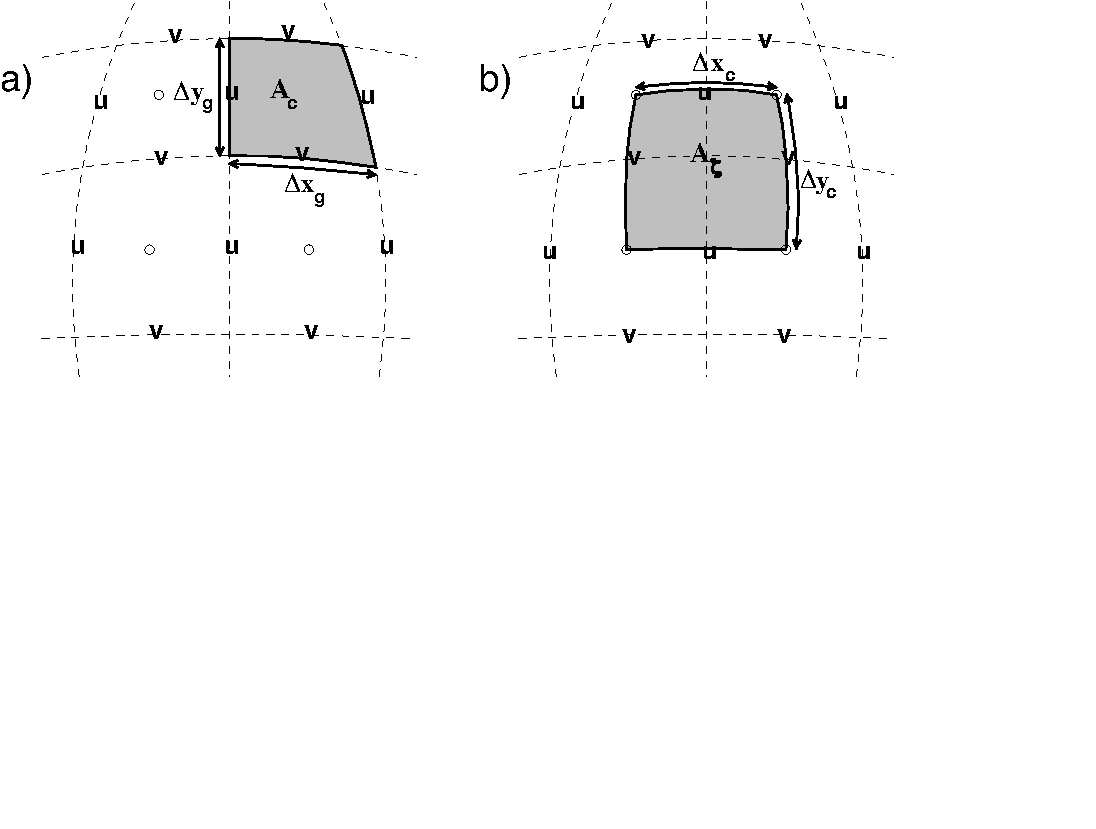
\includegraphics[width=.6\textwidth]{../figures/hgrid-abcd.pdf}
    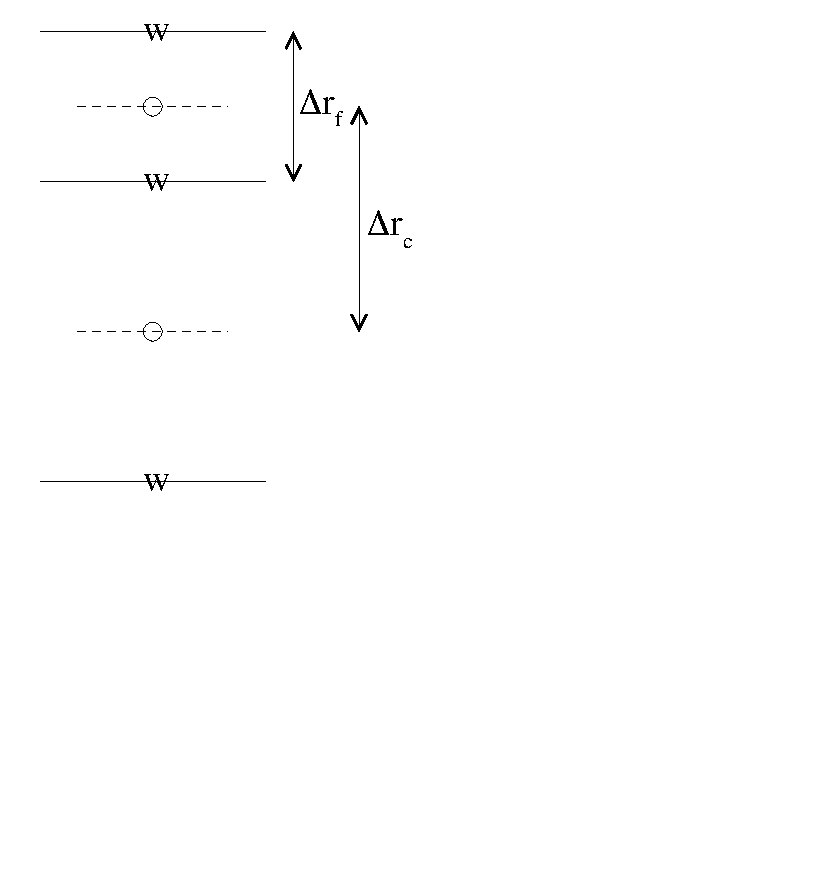
\includegraphics[width=.2\textwidth]{../figures/vgrid-accur-center.pdf}
    \caption{The structured finite volume grid used in the MITgcm. The
        left two figures show the horizontal grid, viewed from above. The right
        figure shows the vertical grid. In each figure, u, v, and w mark the
        location where velocities exist on the grid cell interfaces. The open
        circles denote the tracer location at the grid cell center,
        where fields like temperature and salinity are located. Figures are from
    \citet{campin_mitgcmmitgcm_2021}.}
    \label{fig:mitgcm_grid}
\end{figure}

Starting with the first term,
\begin{linenomath*}\begin{equation*}
    \delta_\jk \coloneqq \dfrac{1}{\vol_\jk}\int_{\cell_\jk}\delta(\x)\,d\x
\end{equation*}\end{linenomath*}
so that
\begin{linenomath*}\begin{equation*}
    \int_{\cell_\jk} \delta(\x)\,\uni(\x)\, d\x =
    \vol_\jk\,\delta_\jk\,\uni_\jk
\end{equation*}\end{linenomath*}
where $\vol_\jk = \Delta y^{j}_{g} \Delta r_f^k$ is the grid cell volume,
indicated by Figure \ref{fig:mitgcm_grid}.
We note that a cartesian style notation
is used, but spherical polar coordinates are used in the computation, and the
MITgcm supports generic curvilinear coordinates.
Generally, the coordinate directions $(x,y,z)$ correspond to $(\lambda,\phi,r)$,
i.e. longitude, latitude, and height.
In the spherical polar case, the differential elements are
\begin{linenomath*}\begin{equation*}
    \Delta x = r_0 \cos(\phi)\Delta\lambda \qquad
    \Delta y = r_0 \Delta \phi \qquad
    \Delta z = \Delta r
\end{equation*}\end{linenomath*}
where $r_0 = 6,378$ km is the nominal radius of the earth, and note that in this
coordinate system latitude $\phi$ is defined to be 0 at the equator.

The third term is, from the definition of a white noise process
\citep{adler_random_2007},
\begin{linenomath*}\begin{equation*}
    \int_{\cell_\jk}\defdet^{-1/2}\W(\x) \, d\x
        = \sqrt{\dfrac{\vol_\jk}{\defdetd}} z_\jk
\end{equation*}\end{linenomath*}
where $z_\jk$ is an uncorrelated (independent) standard Gaussian at each grid
cell center $\jk$, and we used:
\begin{linenomath*}\begin{equation*}
    \defdetd \coloneqq
    \dfrac{1}{\vol_\jk}\int_{\cell_\jk}\defdet\,d\x\,.
\end{equation*}\end{linenomath*}

The second term, containing the Laplacian is handled as follows
\begin{linenomath*}\begin{equation*}
    \int_{\cell_\jk} \nabla\cdot K(\x)\nabla\,\uni(\x)\,d\x
    =\int_{\cellbdy_\jk} K(\x)\nabla\,\uni(\x)\,
    \cdot \hat{\mathbf{n}} \, d\s
\end{equation*}\end{linenomath*}
where $\hat{\mathbf{n}}$ is an outward normal to the cell boundary
$\cellbdy_\jk$.
Throughout this work, we assume the tensor $K(\x)$ to be represented as the
diagonal matrix:
\begin{linenomath*}\begin{equation*}
    K(\x) =
    \begin{pmatrix}
        \kappa^{vy}(\x) & 0 \\
        0 & \kappa^{wz}(\x) \\
    \end{pmatrix} \, .
\end{equation*}\end{linenomath*}
Our choice here is discussed later, and could be generalized in future work.
We represent the
discretized form of this tensor as
\begin{linenomath*}\begin{equation*}
    K_\jk =
    \begin{pmatrix}
        \kappa^{vy}_\jk & 0 \\
        0 & \kappa^{wz}_\jk \\
    \end{pmatrix} \, ,
\end{equation*}\end{linenomath*}
where the elements $\kappa^{vy}_\jk$ and $\kappa^{wz}_\jk$
are located at the $v$ and $w$ grid cell locations in Figure
\ref{fig:mitgcm_grid}.
Additionally
\begin{linenomath*}\begin{equation*}
    \kappa^{vy}_{\jk} \coloneqq \dfrac{1}{\Delta r_f^{\jk}}
    \int_{\cellbdy_{\jk}^{S}} \kappa^{vy}(\x)\,d\x
    \qquad
    \kappa^{wz}_{\jk} \coloneqq \dfrac{1}{\Delta y_g^{\jk}}
    \int_{\cellbdy_{\jk}^{B}} \kappa^{wz}(\x)\,d\x
\end{equation*}\end{linenomath*}
where $\cellbdy_{\jk}^{S}$ and $\cellbdy_{\jk}^{B}$ are the
southern and bottom boundaries of the grid cell.
The discretized gradient is approximated via the finite difference
directional derivative at each cell face:
\begin{linenomath*}\begin{equation*}
    \begin{aligned}
%        \pderiv{\uni}{x}(\x_\jk^W)
%        &\simeq \dfrac{\uni_\jk - \uni_\imjk}{\Delta x_c^\jk}
%        \qquad
%        \pderiv{\uni}{x}(\x_\jk^E)
%        &&\simeq \dfrac{\uni_\ipjk - \uni_\jk}{\Delta x_c^\ipjk}
%        \\
        \pderiv{\uni}{y}(\x_\jk^S)
        &\simeq \dfrac{\uni_\jk - \uni_\jmk}{\Delta y_c^\jk}
        \qquad
        \pderiv{\uni}{y}(\x_\jk^N)
        &&\simeq \dfrac{\uni_\jpk - \uni_\jk}{\Delta y_c^\jpk}
        \\
        \pderiv{\uni}{z}(\x_\jk^B)
        &\simeq \dfrac{\uni_\jk - \uni_\jkm}{\Delta z_c^\jk}
        \qquad
        \pderiv{\uni}{z}(\x_\jk^T)
        &&\simeq \dfrac{\uni_\jkp - \uni_\jk}{\Delta z_c^\jkp}
    \end{aligned}
\end{equation*}\end{linenomath*}
for the south, north, bottom, and top cell faces, respectively.
Putting these definitions together,
\begin{linenomath}\begin{equation}
    \begin{aligned}
        \int_{\cellbdy_\jk}
        &K(\x)\nabla\,\uni(\x)\,
        \cdot \hat{\mathbf{n}} \, d\s
        \coloneqq \\
%        &\left[
%            \left(
%            \dfrac{\kappa^{ux} \, \Delta y_g \Delta r_f}{\Delta x_c}
%            \right)_\ipjk \,
%            (\uni_\ipjk - \uni_\jk) -
%            \left(
%            \dfrac{\kappa^{ux} \, \Delta y_g \Delta r_f}{\Delta x_c}
%            \right)_\jk \,
%            (\uni_\jk - \uni_\imjk)
%        \right]+
%        \\
        &\left[
            \left(
            \dfrac{\kappa^{vy} \, \Delta r_f}{\Delta y_c}
            \right)_\jpk \,
            (\uni_\jpk - \uni_\jk) -
            \left(
            \dfrac{\kappa^{vy} \, \Delta r_f}{\Delta y_c}
            \right)_\jk \,
            (\uni_\jk - \uni_\jmk)
        \right]+
        \\
        &\left[
            \left(
            \dfrac{\kappa^{wz} \, \Delta y_g}{\Delta r_c}
            \right)_\jkp \,
            (\uni_\jkp - \uni_\jk) -
            \left(
            \dfrac{\kappa^{wz} \, \Delta y_g}{\Delta r_c}
            \right)_\jk \,
            (\uni_\jk - \uni_\jkm)
        \right]
        \, .
    \end{aligned}
    \label{eq:big_laplacian}
\end{equation}\end{linenomath}
With each term in equation \eqref{eq:spde_integral} defined above, we have the system of
equations in matrix form:
\begin{linenomath}\begin{equation}
    \begin{aligned}
        (D_\delta - L) \unis &= D_z\mathbf{z}\\
        A\unis &= D_z\mathbf{z}
    \end{aligned}
    \label{eq:fv_spde}
\end{equation}\end{linenomath}
where we have (left) divided by grid cell volume so that:
\begin{linenomath*}\begin{equation*}
    \begin{aligned}
        D_\delta \coloneqq \text{diag}\{\delta_i\}_{i=1}^{\nuni} \qquad
        D_z \coloneqq \text{diag}\left\{
            \dfrac{1}{\sqrt{\vol_i \,\, \defdetdi}}
            \right\}_{i=1}^{\nuni}
    \end{aligned}
\end{equation*}\end{linenomath*}
where for notational simplicity we index each grid cell with $i$, rather than
$j$ and $k$ as above.
Finally, $L$ is defined by appropriately gathering terms in
equation \eqref{eq:big_laplacian}, applying the boundary conditions discussed in the next
subsection, and left dividing by grid cell volume.

At last, the covariance matrix associated with the vector $\unis$ can be
obtained by considering the joint probability distribution of
$\mathbf{z}\sim\mathcal{N}(0,I)$ and
the relation $\mathbf{z} = D_z^{-1}A\unis$, obtained from
equation \eqref{eq:fv_spde}.
That is,
\begin{linenomath*}\begin{equation*}
    \begin{aligned}
        \pi(\mathbf{z})
        &\propto  \exp\left\{-\dfrac{1}{2}\mathbf{z}^T\mathbf{z}\right\} \\
        &\propto \exp\left\{-\dfrac{1}{2}\unis^T A D_z^{-2} A \unis\right\} \\
        &\propto \pi(\unis) \, ,
    \end{aligned}
\end{equation*}\end{linenomath*}
where we note that $A=A^T$.
Thus, we define the differential operator for our covariance model as
\begin{linenomath*}\begin{equation*}
    C \coloneqq A^{-1} D_z \, .
\end{equation*}\end{linenomath*}
\\

\noindent\textbf{Neumann boundary conditions.}
So far we have omitted the discussion of boundaries for the sake of
simplicity.
We employ the Neumann boundary condition:
\begin{linenomath*}\begin{equation*}
    K(\x)\nabla\uni(\x) \cdot \hat{\mathbf{n}} = 0 \qquad \x\in\groundBdy \, .
\end{equation*}\end{linenomath*}
which are implemented in equation \eqref{eq:big_laplacian}
simply by zeroing out the gradient term at solid boundaries.
We note that this has an impact on the covariance structure that is discussed
more concretely with the numerical results in
section \ref{sec:matern_pig}.\\

\noindent\textbf{Generic form of the covariance.}
With the Mat\'ern covariance operator $C$ defined, we recall that
\begin{linenomath*}\begin{equation*}
    \Gamma_{\uni} = \Gamma_{\uni}^{1/2}\Gamma_{\uni}^{T/2}
    = \Sigma X C C^T X \Sigma \, ,
\end{equation*}\end{linenomath*}
and all that is left to define are the operators $X$ and $\Sigma$.
We reserve the definition of $\Sigma$ to
chapter xx, as this becomes somewhat specific to our
application.
Recall that $X$ is defined through the pointwise marginal variance of the
covariance operator $C$.
This can feasibly be computed as $\mathbf{e}_i^TCC^T\mathbf{e}_i$, with
$\mathbf{e}_i$ being the canonical basis vector associated with the $i$th
element of the grid.
However, we compute an approximation based on samples from the covariance model, as
suggested in \citet{weaver_correlation_2001} (and references therein).
Samples of the Gaussian random variable with mean $\unis_0$ and covariance
$C C^T$ are computed as
\begin{linenomath*}\begin{equation*}
    \unis = \unis_0 + C\mathbf{z} \, .
\end{equation*}\end{linenomath*}
We find $X$ by computing the standard deviation from a sample size of $N=1000$.
We note that using this approach to approximate the variance of $C$ scales well
to higher dimensional applications.
Additionally, this approach fits well into our computational framework, since
computing these random samples is a necessary first step for the randomized
eigenvalue decomposition algorithm that is fundamental to our inference problem.


\section{Appendix A: A Block Successive Over Relaxation Method}
\label{sec:block_sor}

Applying the Mat\'ern type prior covariance operator, $C$
requires the solution to an elliptic equation.
We outline here a block-Successive Over Relaxation (SOR) method that was
implemented to solve this problem.
We first make a few notes regarding why we chose this algorithm, and why it had
to be implemented at all.

For better or for worse, the MITgcm is a standalone package, and any code
modifications must not rely on outside packages in order to be incoroporated in
the main distribution.\footnote{The notable exception being the expensive,
    proprietary algorithmic differentiation software TAF \citep{giering2005}
    that is tightly interwoven into the code to enable the adjoint model.}
Therefore, incorporating a solver from e.g.\ \texttt{PETSc} is not allowed.
The MITgcm does contain a conjugate gradient solver, but this relies on
a preconditioning that is motivated by geophysical fluid dynamics that may not
be relevant to the more general Mat\'ern SPDE structure.
Thus, we use the SOR method as it is generally easy to implement, and is ``fast
enough'' noting that the computational cost of most elliptic solvers will be
inconsequential when compared to the time-dependent forward model.

The SOR method is an iterative method for solving $A\mathbf{x} = \mathbf{b}$.
At iteration $k$, the elements of $\mathbf{x}$ are $x_i^k$ (similar
notation for other variables), and we seek the update:
\begin{equation}
    \tilde{x}_i^{k+1} = (1-\omega) x_i^k + \dfrac{\omega}{a_{ii}}
    \left( b_i - \sum_{j<i}a_{ij}\tilde{x}_j^{k+1} -
        \sum_{j>i}a_{ij}x_j^{k}\right), \qquad
        i=1,2,...,N \, ,
    \label{eq:sor_update}
\end{equation}
where $\omega$ is the SOR parameter.
We compare this method to the standard Jacobi update
$$\tilde{x}_i^{k+1} = x_i^k + \sum_{i\ne j}\dfrac{a_{ij}x_j^k}{a_{ii}}, \qquad
i=1,2,...,N \, .$$
Here the notation $\tilde{x}_i^{k+1}$ refers to the fact this is a local update,
i.e. there is no communication between the processes assigned to each portion of
the computational domain.
The only areas where this local update causes the algorithm to deviate from a
true SOR method is where neighboring elements
$\tilde{x}^{k+1}_{j}, i\ne j$ are in the ``halo'' regions (i.e. outside of a
process's subdomain).
In this case, $\tilde{x}^{k+1}_j = x^k_j$.

\begin{figure}
    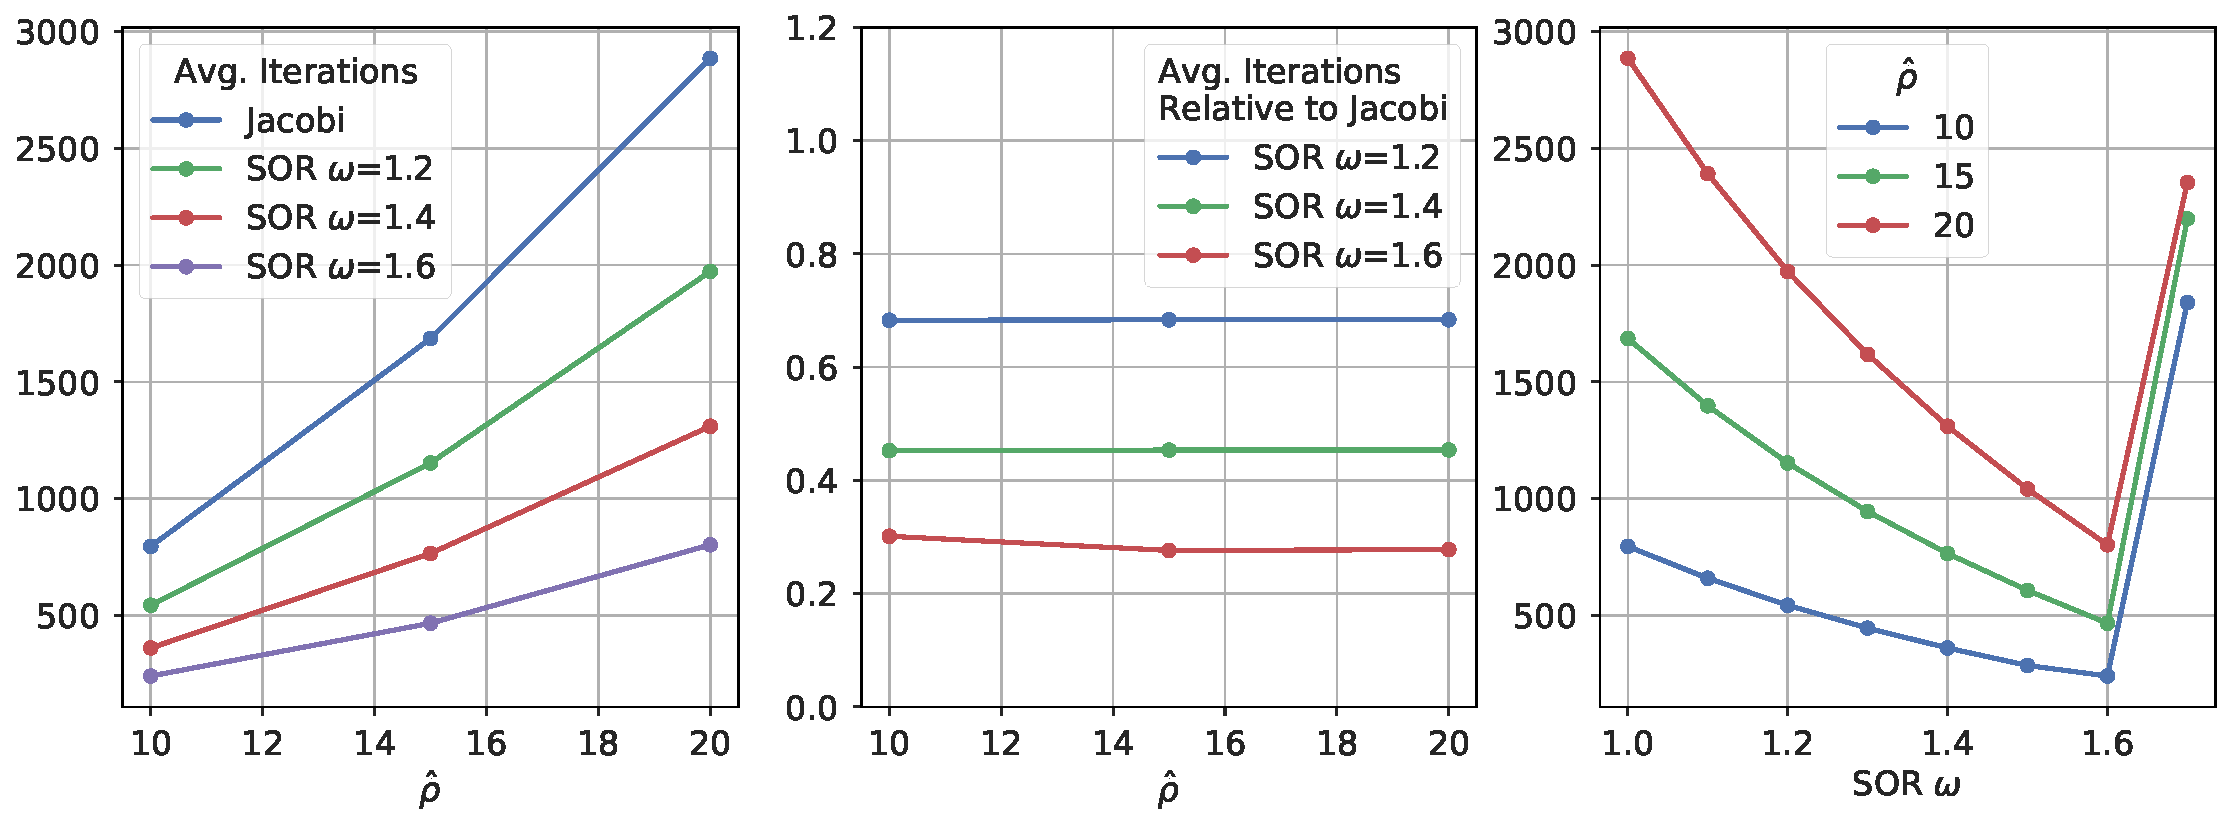
\includegraphics[width=\textwidth]{../figures/sor_noXi.pdf}
    \caption{Performance of the SOR algorithm for various settings of $\omega$.
        Average number of SOR or Jacobi iterations to convergence are shown
        based on solving equation \eqref{eq:fv_spde} with 1000 samples from a
        standard normal as the right hand side. Here $\xi=1$.}
    \label{fig:sor}
\end{figure}

We find this simple modification to be an effective means of speeding up the
linear solve.
Figure \ref{fig:sor} shows that the number of iterations required for
convergence is reduced to about 30\% of the Jacobi scheme.
Of course, a major drawback of the SOR algorithm is exhibited here as well: the
efficiency is highly sensitive to the parameter $\omega$, as shown in
right panel of Figure \ref{fig:sor}.
We
additionally find the performance to be dependent on the length scales used in the Jacobian
$\defjac$, defined in section \ref{sec:matern_operator}.
To facilitate the discussion, we define $L_y = \xi \Delta y$, where $\xi$ is
some multiple that accentuates length scales further in the meridional direction
(e.g.\ $\xi=2$ in many of the results shown in this work).
The vertical length scale is kept the same as before, i.e.\ $L_z = \Delta r$.
We report here that the optimal SOR parameter depends on $\xi$, as shown in
Figure \ref{fig:sor}, and
the optimal parameter for each $\xi$ tested is shown in
Table \ref{table:sor_xi}.
As $\xi$ increases, $\omega^*\rightarrow 1$, and the algorithm approaches
the standard Jacobi algorithm.

\begin{table}[]
    \centering
    \caption{Optimal SOR parameter $\omega^*$ as a function of
        $\xi$, where $L_y = \xi \Delta y$.}
    \label{table:sor_xi}
    \begin{tabular}{c|c|c|c|c}
                   & $\xi=1/2$ & $\xi=1$ & $\xi=2$ & $\xi=5$ \\ \hline
        $\omega^*$ & 1.8 & 1.6 & 1.3 & 1.2                   \\
\end{tabular}
\end{table}

Finally, we note that in the current implementation of this algorithm we update
the ``halo'' regions of $\x$, i.e. $\tilde\x\rightarrow\x$, at the end of each iteration in the
solver.
We recognize that performance could be improved further by
increasing the number of iterations taken before updating the halo regions,
in to reduce communication.
This possible performance benefit could be explored in future work.


%\section{Application to the Pine Island ice shelf domain}
\label{sec:matern_pig}

Here we show the implementation of the covariance model within the MITgcm,
using the computational grid that we will employ to study the Pine Island cavity
circulation.
We discuss more details on how the grid is obtained in
chapter xx.
However, we mention that the horizontal grid scale is
approximately $\Delta x \simeq \Delta y \simeq 600$~m, and the vertical grid
scale is $\Delta r = 20$~m.
Finally, we note that applying $C$ to a random gaussian vector $\mathbf{z}$
requires the solution to an inverse elliptic operator,
which we obtain with an implementation of a block-Successive Over Relaxation
(SOR) method.
The MITgcm uses no external packages, so interfacing with
e.g.\ \texttt{PETSc} is not an option for any code that is meant to be
contributed to the main MITgcm distribution - which is our intention.
While the solver is far from perfect, it provides decent performance and is
easy to implement.
We discuss details of the implementation and
performance in xx. \\

\noindent\textbf{Samples from the covariance model.}
Figure \ref{fig:matern_samples} (top row) shows samples from the normalized
covariance at the western open boundary of the computational domain,
$XC\mathbf{z}$.
In all cases we use $L_y = 2\Delta y$ and $L_z = \Delta r$, so correlation
length scales vary purely by the specification of $\rangeh$.
The approximate length scale associated with $\rangeh$ is indicated by the arrows on
the bottom right corner of each plot, which qualitatively compares well to the
structure of the random samples.
We note that their is high anisotropy in the domain:
the meridional extent at $Z=0$ (i.e. non-gray distance along the x-axis at the
top of each figure) is $\sim$73~km, while the maximum depth is $\sim1$~km.

The random samples in Figure \ref{fig:matern_samples} (top row)
are normalized by $X$ to have approximately unit variance.
The pointwise marginal standard deviation, $\hat{\sigma}$, which is the inverse
of the diagonal elements of $X$, is shown in Figure \ref{fig:matern_samples}
(bottom row).
With larger correlation length scales, the standard deviation of $C$ increases.
This is particularly true near the boundaries of the field, where we see narrow
bathymetric trenches extending to depth.\\

\begin{figure}
    \centering
    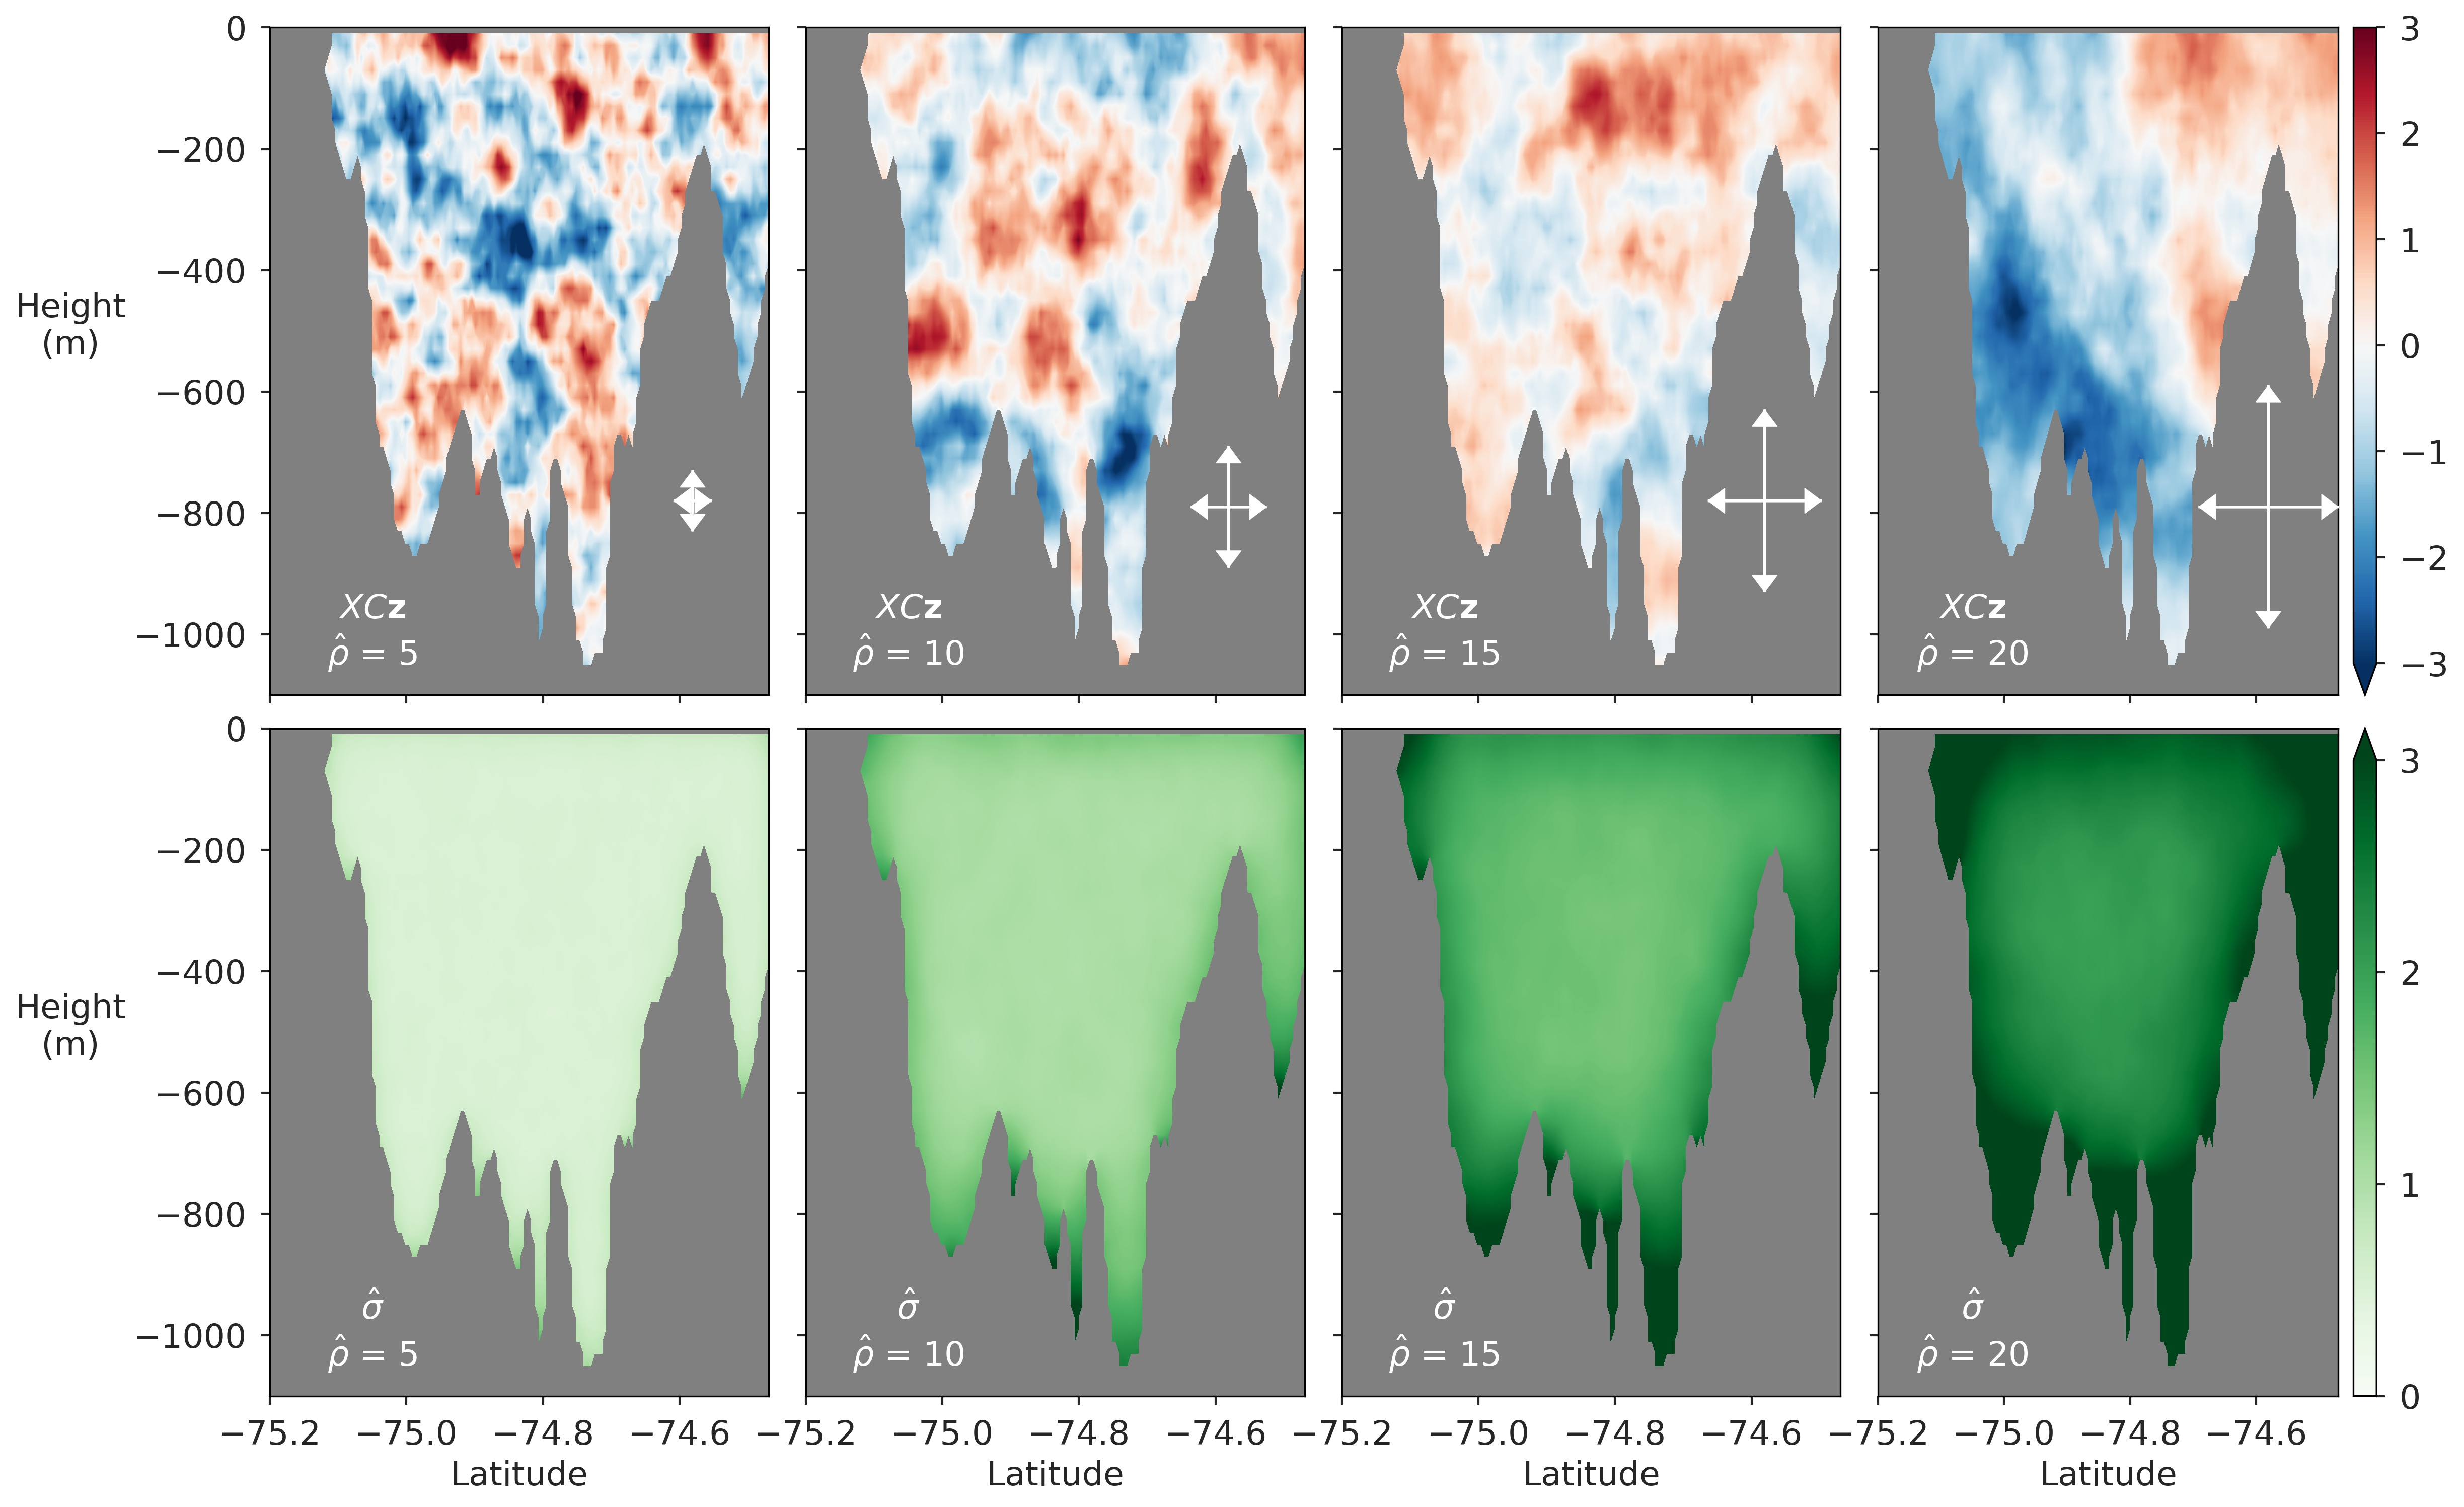
\includegraphics[width=\textwidth]{../figures/samples_and_pointwise_std.jpg}
    \caption{Normalized samples and pointwise standard deviation from the covariance
        model.
        (top row) Samples from the covariance model, normalized by the
        pointwise standard deviation. Each column shows increasing correlation
        length scales, which is regulated by $\rangeh$.
        The arrows in the bottom right corner of each plot show the approximate length scales
        that are covered by $\rangeh L_y$ and $\rangeh L_z$, respectively.
        Here we have used $L_y = 2\Delta y_g$ and $L_z=\Delta r_f$, see
        Figure \ref{fig:mitgcm_grid} for a notational reference.
        We note that the standard normal vector $\mathbf{z}$ is unique in
        each figure.
        (bottom row) Pointwise standard deviation of the covariance operator
        $CC^T$, estimated from
        a sample size of $N=1000$. The diagonal matrix $X$ is comprised of the
        inverse of this field.
    }
    \label{fig:matern_samples}
\end{figure}


\noindent\textbf{Correlation length scales.}
Here we show that the correlations obtained from random samples agree well with
the structure that one would expect from the Mat\'ern model.
We consider the correlation function associated with the isotropic Mat\'ern
covariance from equation \eqref{eq:matern_covariance_iso}:
\begin{equation*}
    \begin{aligned}
        r(\rangeh,\xh_1,\xh_2) &= r(\rangeh, ||\xh_1-\xh_2||) \\
                       &= c(\xh_1,\xh_2)/\sigma^2 \\
                       &= \dfrac{1}{2^{\meandiff-1}\mathcal{G}(\meandiff)}
        \left(\dfrac{\sqrt{8\meandiff}}{\rangeh} ||\xh_2-\xh_1||\right)^\meandiff
        \mathcal{B}_\meandiff
        \left(\dfrac{\sqrt{8\meandiff}}{\rangeh} ||\xh_2-\xh_1||\right) \, ,
    \end{aligned}
\end{equation*}
which emphasizes that correlation is determined purely by Euclidean distance in
the transformed space.

We compare correlation distances in the computational domain to the
theoretical value, $r(\rangeh,||\xh_1-\xh_2||)$, by using the mapping method described in
section \ref{sec:matern_review}.
Specifically, we compute the correlation coefficient from the random samples
used to approximate $X$ as a function of distance in the computational domain.
We then map these distances back to the ``transformed'' space $\defdomain$ via
the inverse map $\defmap^{-1}$.
We note that $\defmap$ has a differentiable inverse $\defmap^{-1}$ by construction
through the inverse function theorem,
as a result of defining $\defmap$ through its Jacobian $\defjac$ such that
$\defdet \neq 0 \,\,\forall \,\,\x\in\openBdy$.
Specifically, distances in the computational domain are mapped to the
transformed space for arbritrary points $\x_1,\x_2\in\openBdy$ such that
$\xh_1\coloneqq\defmap^{-1}(\x_1)$ and $\xh_2\coloneqq \defmap^{-1}(\x_2)$ as
follows:
\begin{equation*}
    \begin{aligned}
        \xh_2 - \xh_1 &= \defmap^{-1}(\x_2) - \defmap^{-1}(\x_1) \\
                      &= \left(
                            \defmap^{-1}(\x_1) +
                            \defjac^{-1}\big|_{\x_{1}}(\x_2-\x_1) +
                            \bigo( ||\x_2-\x_1|| )
                        \right) - \defmap^{-1}(\x_1) \\
                        &\simeq \defjac^{-1}\big|_{\x_{1}}(\x_2-\x_1) \, .
    \end{aligned}
    \label{eq:matern_correlation_iso}
\end{equation*}
That is, we use the inverse Jacobian to map distances in the computational domain to the
transformed space $\defdomain$, where we can compare correlation statistics to
the Mat\'ern formula.
We make one final approximation to ease the process.
In the spherical polar coordinate system used, recall that
$\Delta y = r_0 \Delta \phi$, i.e. the meridional grid spacing varies with
latitude.
However, the meridional extent of our computational domain is relatively small,
such that $\Delta y$ only varies from $\sim 582-620$~m.
We therefore assume that
$\defjac^{-1}\big|_{\x_{1}} =\defjac^{-1}\,\,\forall\,\,\x_1\in\openBdy$
simply for the sake of this calculation.

The sample correlation coefficent computed from the 1000 random samples are
shown for various values of $\rangeh$ in Figure \ref{fig:matern_correlations}.
We separately compute distances in the meridional (left panel) and vertical
(right panel) directions as
\begin{equation*}
    \delta \hat{y} = \defjac^{-1}\delta y
    \qquad
    \delta \hat{z} = \defjac^{-1}\delta z \, .
\end{equation*}
Each colored curve shows the domain averaged correlation coefficient for a
particular $\rangeh$, and the spread denotes one standard deviation above and
below the mean.
Each black curve shows the theoretical, predicted correlation for the distances
in the deformed space $\delta\hat{y}$ and $\delta\hat{z}$.
At larger values of $\rangeh$, the spread in correlation coefficient and
mismatch between the theoretical prediction grow larger.
We attribute this to boundary effects, and note that this slice of the
computational domain has at its maximum extent 60~$L_y$ and 53~$L_z$.
Thus, we expect some degree of difference between the SPDE derived correlation
and the functional form of the covariance model.
However, in general we find the agreement to be quite good.
The result is that we can formulate the covariance model (i.e.\ choose
$\rangeh$) based on our intuition from the simple isotropic form, and this is
easily mapped to the computational domain.

\begin{figure}
    \centering
    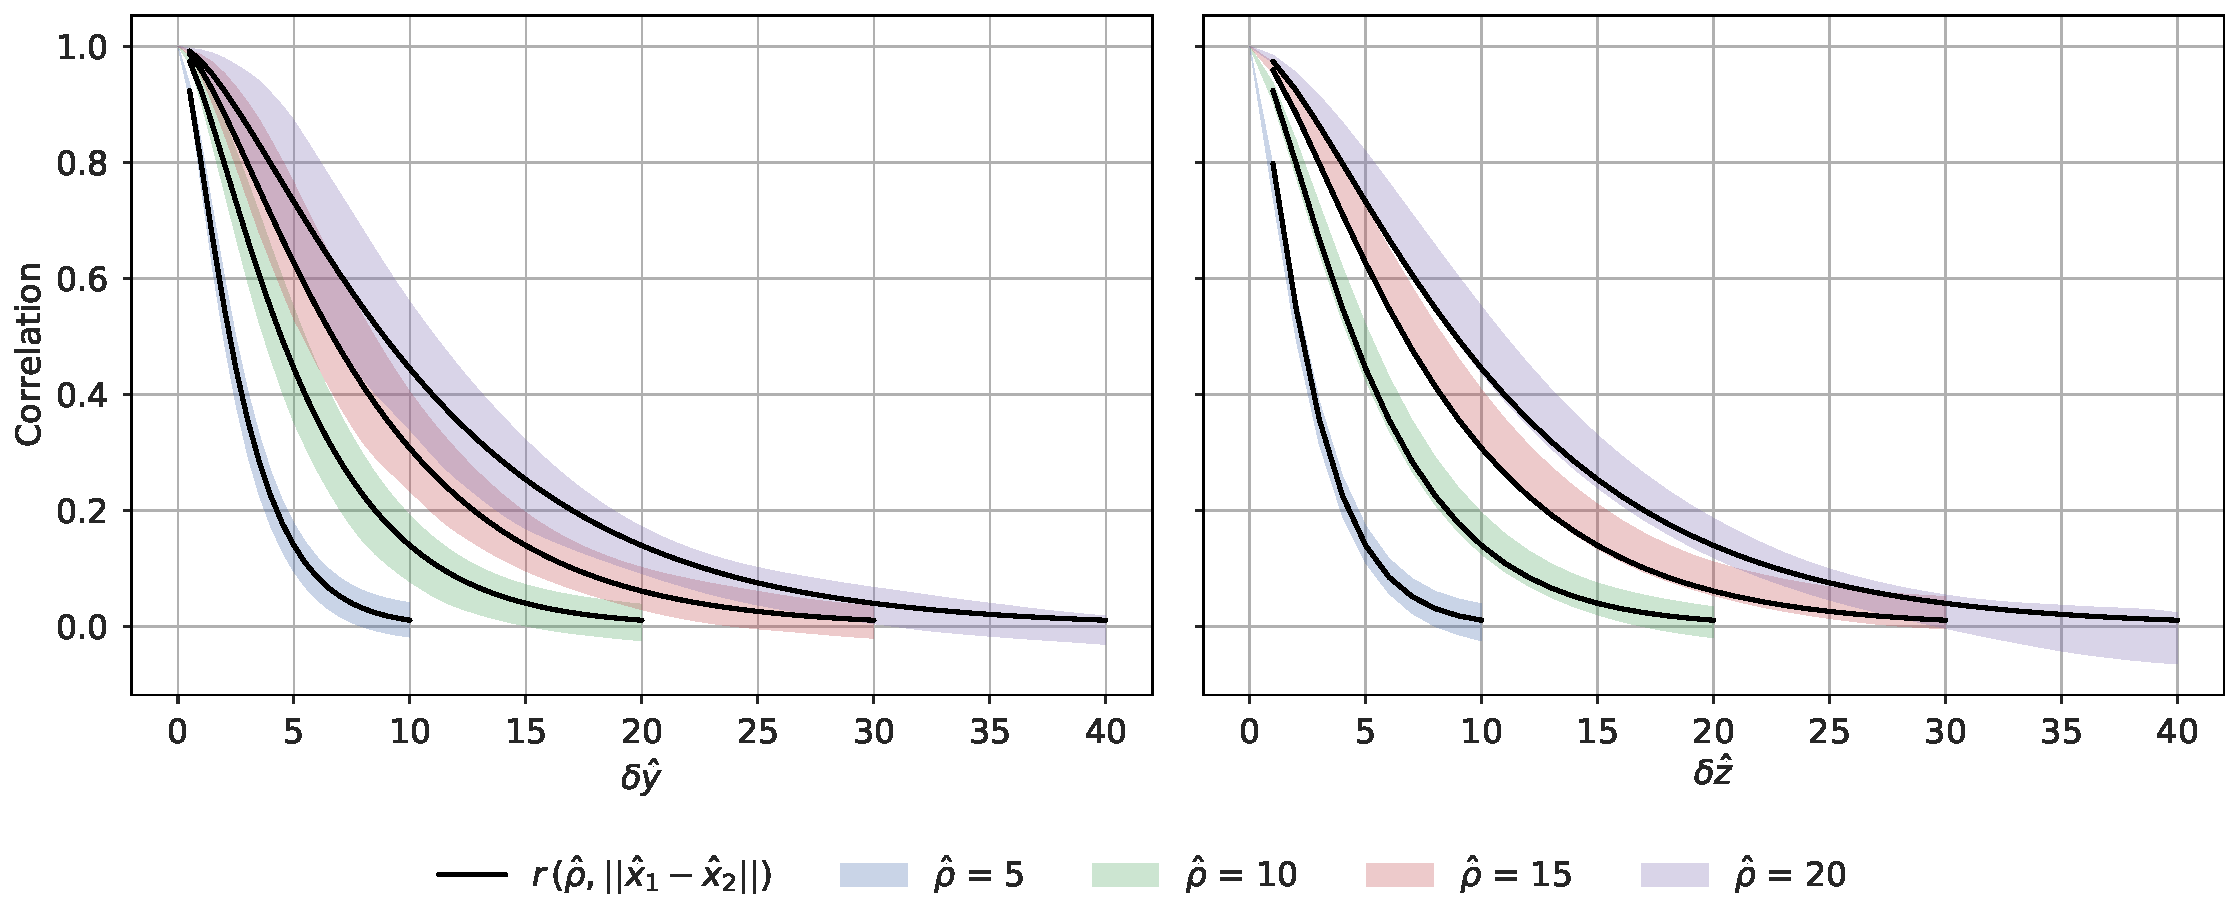
\includegraphics[width=\textwidth]{../figures/nondimensional_correlation.pdf}
    \caption{Correlation coefficient corresponding to different distances in the
        (left) meridional and (right) vertical directions. The coefficient is
        computed from the random samples used to estimate
        $\hat{\sigma}$ and $X$. Each color denotes correlations computed for a
        different value of $\rangeh$, and the spread is determined by one standard
        deviation around the domain averaged correlation coefficent.
        The black curve denotes the predicted isotropic correlation predicted by
        equation \eqref{eq:matern_correlation_iso} with the appropriate value for
        $\rangeh$.}
    \label{fig:matern_correlations}
\end{figure}



\acknowledgments
Thanks everyone.

\bibliography{references}
\end{document}
